\documentclass{whiteboard}
\begin{document}
\begin{frame}[plain,t]
\bbcover{Grafos}{Algoritmo de Floyd-Warshall}{Prof. Edson Alves}{Faculdade UnB Gama}

\end{frame}
\begin{frame}[plain,t]
\begin{tikzpicture}
\node[draw,opacity=0] at (0, 0) {x};
\node[draw,opacity=0] at (14, 8) {x};

	\node[] (floyd) at (2.0, 5.0) { \includegraphics[scale=0.4]{figs/floyd.jpg} };

	\node[] (fname) at (2.0, 2.75) { \bbbold{Robert W. Floyd} };

	\node[] (fdate) at (2.0, 2.25) { \bbtext{(1962)} };


\end{tikzpicture}
\end{frame}
\begin{frame}[plain,t]
\begin{tikzpicture}
\node[draw,opacity=0] at (0, 0) {x};
\node[draw,opacity=0] at (14, 8) {x};

	\node[] (floyd) at (2.0, 5.0) { \includegraphics[scale=0.4]{figs/floyd.jpg} };

	\node[] (fname) at (2.0, 2.75) { \bbbold{Robert W. Floyd} };

	\node[] (fdate) at (2.0, 2.25) { \bbtext{(1962)} };



	\node[] (warshall) at (8.0, 6.0) { \includegraphics[scale=2.4]{figs/warshall.jpg} };

	\node[] (wname) at (11.0, 6.5) { \bbbold{Stephen Warshall} };

	\node[] (wdate) at (11.0, 6.0) { \bbtext{(1962)} };

\end{tikzpicture}
\end{frame}
\begin{frame}[plain,t]
\begin{tikzpicture}
\node[draw,opacity=0] at (0, 0) {x};
\node[draw,opacity=0] at (14, 8) {x};

	\node[] (floyd) at (2.0, 5.0) { \includegraphics[scale=0.4]{figs/floyd.jpg} };

	\node[] (fname) at (2.0, 2.75) { \bbbold{Robert W. Floyd} };

	\node[] (fdate) at (2.0, 2.25) { \bbtext{(1962)} };



	\node[] (warshall) at (8.0, 6.0) { \includegraphics[scale=2.4]{figs/warshall.jpg} };

	\node[] (wname) at (11.0, 6.5) { \bbbold{Stephen Warshall} };

	\node[] (wdate) at (11.0, 6.0) { \bbtext{(1962)} };


	\node[] (roy) at (8.0, 2.0) { \includegraphics[scale=0.1]{figs/roy.jpg} };

	\node[] (rname) at (11.5, 2.5) { \bbbold{Bernard Roy} };

	\node[] (rdate) at (11.5, 2.0) { \bbtext{(1959)} };


\end{tikzpicture}
\end{frame}
\begin{frame}[plain,t]
\begin{tikzpicture}
\node[draw,opacity=0] at (0, 0) {x};
\node[draw,opacity=0] at (14, 8) {x};

	\node[anchor=west] (title) at (0.0, 7.0) { \Large \bbbold{Características do algoritmo de Bellman-Ford} };
\end{tikzpicture}
\end{frame}
\begin{frame}[plain,t]
\begin{tikzpicture}
\node[draw,opacity=0] at (0, 0) {x};
\node[draw,opacity=0] at (14, 8) {x};

	\node[anchor=west] (title) at (0.0, 7.0) { \Large \bbbold{Características do algoritmo de Bellman-Ford} };

	\node[anchor=west] (a) at (0.5, 6.0) { $\star$ \bbtext{Computa o caminho mínimo entre todos os pares de vértices de $G(V, E)$} };

\end{tikzpicture}
\end{frame}
\begin{frame}[plain,t]
\begin{tikzpicture}
\node[draw,opacity=0] at (0, 0) {x};
\node[draw,opacity=0] at (14, 8) {x};

	\node[anchor=west] (title) at (0.0, 7.0) { \Large \bbbold{Características do algoritmo de Bellman-Ford} };

	\node[anchor=west] (a) at (0.5, 6.0) { $\star$ \bbtext{Computa o caminho mínimo entre todos os pares de vértices de $G(V, E)$} };


	\node[anchor=west] (b) at (0.5, 5.0) { $\star$ \bbtext{É capaz de processar arestas negativas} };

\end{tikzpicture}
\end{frame}
\begin{frame}[plain,t]

\begin{tikzpicture}
\node[draw,opacity=0] at (0, 0) {x};
\node[draw,opacity=0] at (14, 8) {x};

	\node[anchor=west] (title) at (0.0, 7.0) { \Large \bbbold{Características do algoritmo de Bellman-Ford} };

	\node[anchor=west] (a) at (0.5, 6.0) { $\star$ \bbtext{Computa o caminho mínimo entre todos os pares de vértices de $G(V, E)$} };


	\node[anchor=west] (b) at (0.5, 5.0) { $\star$ \bbtext{É capaz de processar arestas negativas} };


	\node[anchor=west] (c) at (0.5, 4.0) { $\star$ \bbtext{Não processa, mas identifica ciclos negativos} };

\end{tikzpicture}
\end{frame}
\begin{frame}[plain,t]
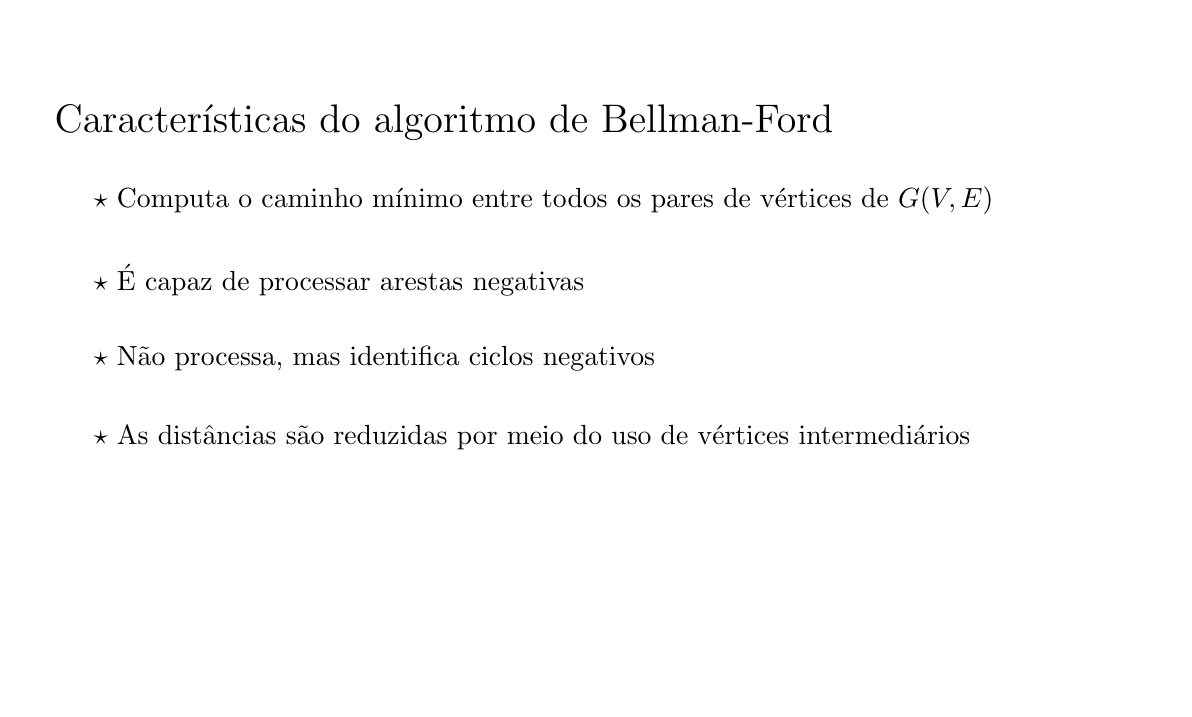
\begin{tikzpicture}
\node[draw,opacity=0] at (0, 0) {x};
\node[draw,opacity=0] at (14, 8) {x};

	\node[anchor=west] (title) at (0.0, 7.0) { \Large \bbbold{Características do algoritmo de Bellman-Ford} };

	\node[anchor=west] (a) at (0.5, 6.0) { $\star$ \bbtext{Computa o caminho mínimo entre todos os pares de vértices de $G(V, E)$} };


	\node[anchor=west] (b) at (0.5, 5.0) { $\star$ \bbtext{É capaz de processar arestas negativas} };


	\node[anchor=west] (c) at (0.5, 4.0) { $\star$ \bbtext{Não processa, mas identifica ciclos negativos} };


	\node[anchor=west] (d) at (0.5, 3.0) { $\star$ \bbtext{As distâncias são reduzidas por meio do uso de vértices intermediários} };

\end{tikzpicture}
\end{frame}
\begin{frame}[plain,t]
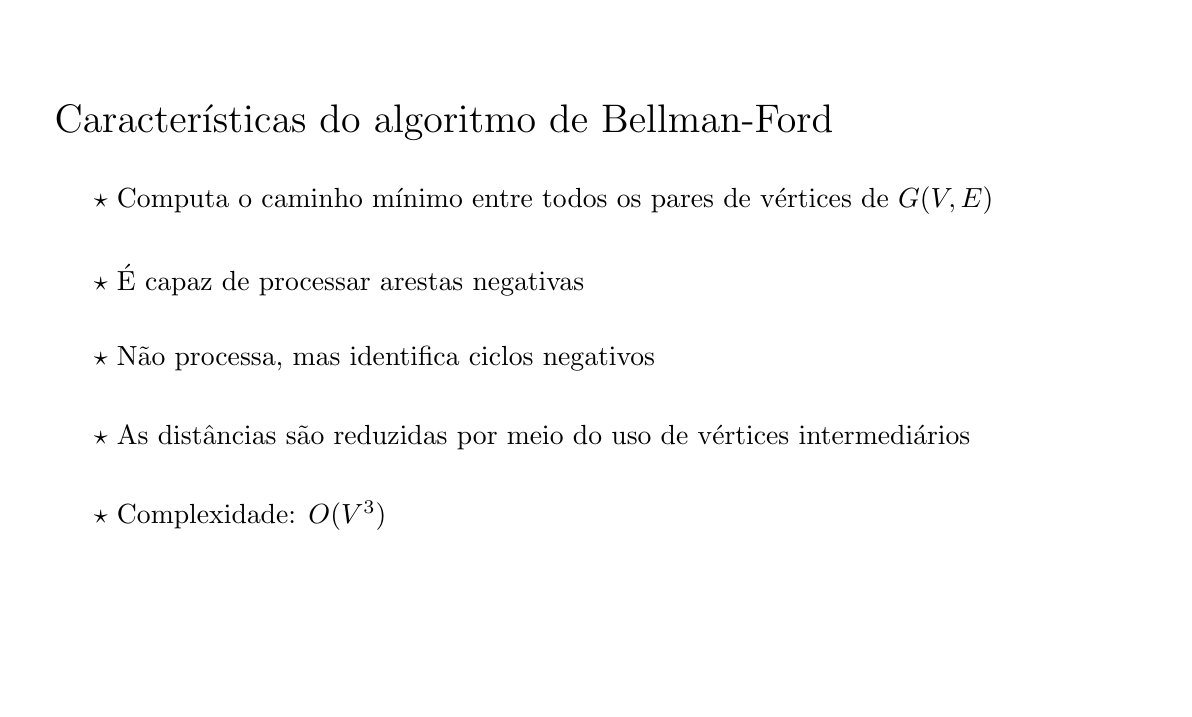
\begin{tikzpicture}
\node[draw,opacity=0] at (0, 0) {x};
\node[draw,opacity=0] at (14, 8) {x};

	\node[anchor=west] (title) at (0.0, 7.0) { \Large \bbbold{Características do algoritmo de Bellman-Ford} };

	\node[anchor=west] (a) at (0.5, 6.0) { $\star$ \bbtext{Computa o caminho mínimo entre todos os pares de vértices de $G(V, E)$} };


	\node[anchor=west] (b) at (0.5, 5.0) { $\star$ \bbtext{É capaz de processar arestas negativas} };


	\node[anchor=west] (c) at (0.5, 4.0) { $\star$ \bbtext{Não processa, mas identifica ciclos negativos} };


	\node[anchor=west] (d) at (0.5, 3.0) { $\star$ \bbtext{As distâncias são reduzidas por meio do uso de vértices intermediários} };


	\node[anchor=west] (e) at (0.5, 2.0) { $\star$ \bbtext{\bbbold{Complexidade}: $O(V^3)$ } };

\end{tikzpicture}
\end{frame}
\begin{frame}[plain,t]
\begin{tikzpicture}
\node[draw,opacity=0] at (0, 0) {x};
\node[draw,opacity=0] at (14, 8) {x};

	\node[anchor=west] (title) at (0.0, 7.0) { \Large \bbbold{Pseudocódigo} };

\end{tikzpicture}
\end{frame}
\begin{frame}[plain,t]
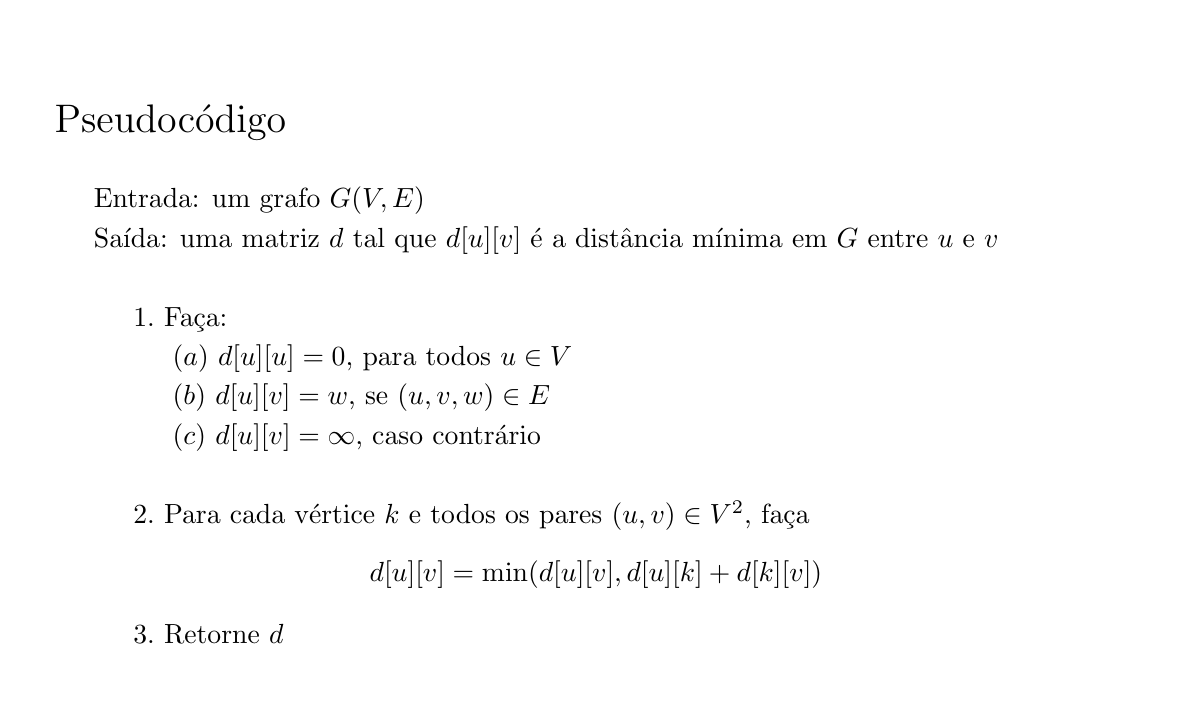
\begin{tikzpicture}
\node[draw,opacity=0] at (0, 0) {x};
\node[draw,opacity=0] at (14, 8) {x};

	\node[anchor=west] (title) at (0.0, 7.0) { \Large \bbbold{Pseudocódigo} };


	\node[anchor=west] (input) at (0.5, 6.0) { \bbemph{Entrada:} \bbtext{um grafo $G(V, E)$} };

	\node[anchor=west] (output) at (0.5, 5.5) { \bbemph{Saída:} \bbtext{uma matriz $d$ tal que $d[u][v]$ é a distância mínima em $G$ entre $u$ e $v$} };

	\node[anchor=west] (step1) at (1.0, 4.5) { $1.$ \bbtext{Faça:} };

	\node[anchor=west] (step1_1) at (1.5, 4.0) { $(a)$ $d[u][u] = 0$, \bbtext{para todos} $u\in V$ };

	\node[anchor=west] (step1_2) at (1.5, 3.5) { $(b)$ $d[u][v] = w$, \bbtext{se} $(u, v, w)\in E$ };

	\node[anchor=west] (step1_3) at (1.5, 3.0) { $(c)$ $d[u][v] = \infty$, \bbtext{caso contrário} };

	\node[anchor=west] (step2) at (1.0, 2.0) { $2.$ \bbtext{Para cada vértice $k$ e todos os pares $(u,v)\in V^2$, faça} };

	\node[] (dist) at (7.0, 1.25) { $d[u][v] = \min(d[u][v], d[u][k] + d[k][v])$ };

	\node[anchor=west] (step3) at (1.0, 0.5) { $3.$ \bbtext{Retorne} $d$ };

\end{tikzpicture}
\end{frame}
\begin{frame}[plain,t]
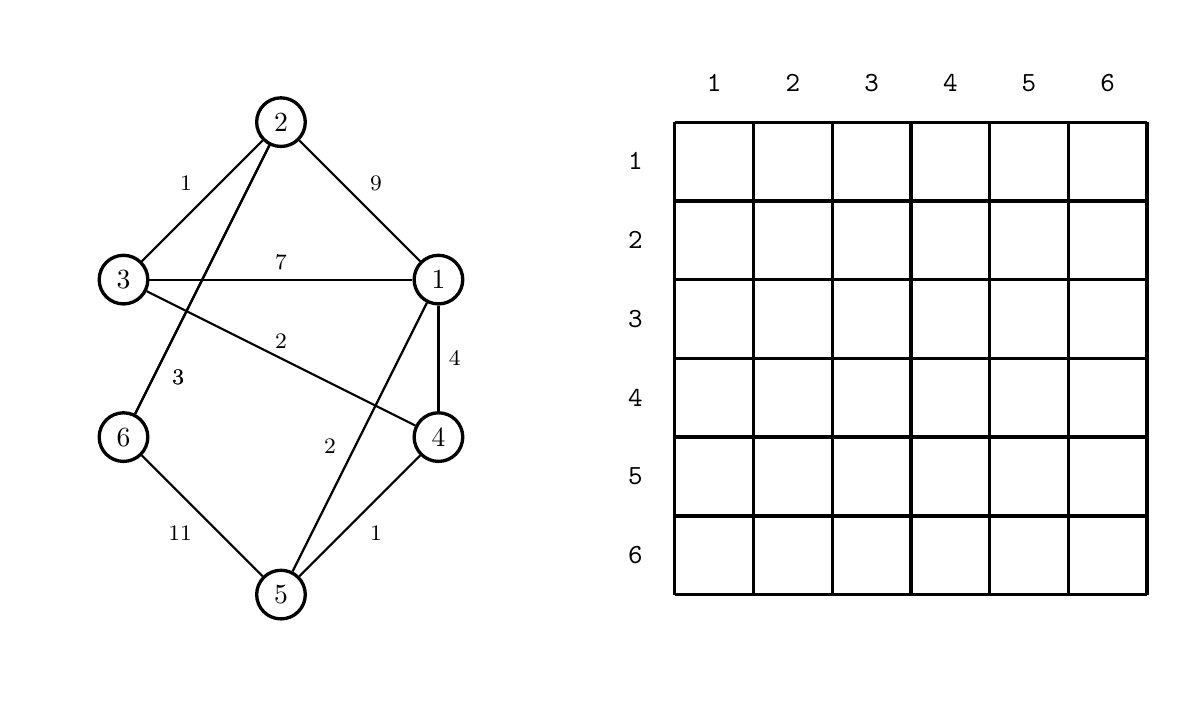
\begin{tikzpicture}
\node[draw,opacity=0] at (0, 0) {x};
\node[draw,opacity=0] at (14, 8) {x};

	\draw[very thick] (8.0, 1.0) grid  (14.0, 7.0);

	\node[] (x1) at (8.5, 7.5) { \bbtext{\tt 1} };

	\node[] (x2) at (9.5, 7.5) { \bbtext{\tt 2} };

	\node[] (x3) at (10.5, 7.5) { \bbtext{\tt 3} };

	\node[] (x4) at (11.5, 7.5) { \bbtext{\tt 4} };

	\node[] (x5) at (12.5, 7.5) { \bbtext{\tt 5} };

	\node[] (x6) at (13.5, 7.5) { \bbtext{\tt 6} };

	\node[] (y1) at (7.5, 6.5) { \bbtext{\tt 1} };

	\node[] (y2) at (7.5, 5.5) { \bbtext{\tt 2} };

	\node[] (y3) at (7.5, 4.5) { \bbtext{\tt 3} };

	\node[] (y4) at (7.5, 3.5) { \bbtext{\tt 4} };

	\node[] (y5) at (7.5, 2.5) { \bbtext{\tt 5} };

	\node[] (y6) at (7.5, 1.5) { \bbtext{\tt 6} };

	\node[very thick,draw,circle] (node1) at (5.0, 5.0) { \bbtext{1} };

	\node[very thick,draw,circle] (node2) at (3.0, 7.0) { \bbtext{2} };

	\node[very thick,draw,circle] (node3) at (1.0, 5.0) { \bbtext{3} };

	\node[very thick,draw,circle] (node4) at (5.0, 3.0) { \bbtext{4} };

	\node[very thick,draw,circle] (node5) at (3.0, 1.0) { \bbtext{5} };

	\node[very thick,draw,circle] (node6) at (1.0, 3.0) { \bbtext{6} };

	\draw[thick](node1) to node[above right] {\footnotesize \bbinfo{9}} (node2);

	\draw[thick](node1) to node[above] {\footnotesize \bbinfo{7}} (node3);

	\draw[thick](node1) to node[right] {\footnotesize \bbinfo{4}} (node4);

	\draw[thick](node1) to node[above left,pos=.6] {\footnotesize \bbinfo{2}} (node5);

	\draw[thick](node2) to node[above left] {\footnotesize \bbinfo{1}} (node3);

	\draw[thick](node2) to node[below right,pos=.8] {\footnotesize \bbinfo{3}} (node6);

	\draw[thick](node2) to node[below right,pos=.8] {\footnotesize \bbinfo{3}} (node6);

	\draw[thick](node3) to node[above] {\footnotesize \bbinfo{2}} (node4);

	\draw[thick](node4) to node[below right] {\footnotesize \bbinfo{1}} (node5);

	\draw[thick](node5) to node[below left] {\footnotesize \bbinfo{11}} (node6);

\end{tikzpicture}
\end{frame}
\begin{frame}[plain,t]
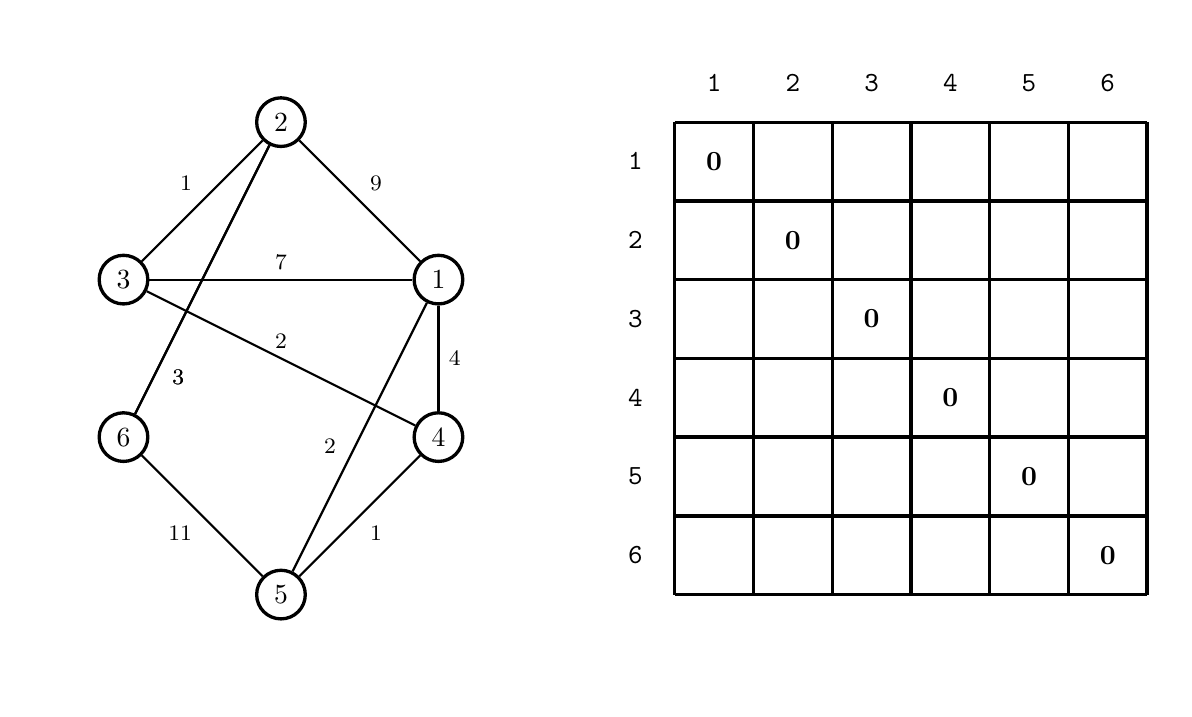
\begin{tikzpicture}
\node[draw,opacity=0] at (0, 0) {x};
\node[draw,opacity=0] at (14, 8) {x};

	\draw[very thick] (8.0, 1.0) grid  (14.0, 7.0);

	\node[] (x1) at (8.5, 7.5) { \bbtext{\tt 1} };

	\node[] (x2) at (9.5, 7.5) { \bbtext{\tt 2} };

	\node[] (x3) at (10.5, 7.5) { \bbtext{\tt 3} };

	\node[] (x4) at (11.5, 7.5) { \bbtext{\tt 4} };

	\node[] (x5) at (12.5, 7.5) { \bbtext{\tt 5} };

	\node[] (x6) at (13.5, 7.5) { \bbtext{\tt 6} };

	\node[] (y1) at (7.5, 6.5) { \bbtext{\tt 1} };

	\node[] (y2) at (7.5, 5.5) { \bbtext{\tt 2} };

	\node[] (y3) at (7.5, 4.5) { \bbtext{\tt 3} };

	\node[] (y4) at (7.5, 3.5) { \bbtext{\tt 4} };

	\node[] (y5) at (7.5, 2.5) { \bbtext{\tt 5} };

	\node[] (y6) at (7.5, 1.5) { \bbtext{\tt 6} };

	\node[very thick,draw,circle] (node1) at (5.0, 5.0) { \bbtext{1} };

	\node[very thick,draw,circle] (node2) at (3.0, 7.0) { \bbtext{2} };

	\node[very thick,draw,circle] (node3) at (1.0, 5.0) { \bbtext{3} };

	\node[very thick,draw,circle] (node4) at (5.0, 3.0) { \bbtext{4} };

	\node[very thick,draw,circle] (node5) at (3.0, 1.0) { \bbtext{5} };

	\node[very thick,draw,circle] (node6) at (1.0, 3.0) { \bbtext{6} };

	\draw[thick](node1) to node[above right] {\footnotesize \bbinfo{9}} (node2);

	\draw[thick](node1) to node[above] {\footnotesize \bbinfo{7}} (node3);

	\draw[thick](node1) to node[right] {\footnotesize \bbinfo{4}} (node4);

	\draw[thick](node1) to node[above left,pos=.6] {\footnotesize \bbinfo{2}} (node5);

	\draw[thick](node2) to node[above left] {\footnotesize \bbinfo{1}} (node3);

	\draw[thick](node2) to node[below right,pos=.8] {\footnotesize \bbinfo{3}} (node6);

	\draw[thick](node2) to node[below right,pos=.8] {\footnotesize \bbinfo{3}} (node6);

	\draw[thick](node3) to node[above] {\footnotesize \bbinfo{2}} (node4);

	\draw[thick](node4) to node[below right] {\footnotesize \bbinfo{1}} (node5);

	\draw[thick](node5) to node[below left] {\footnotesize \bbinfo{11}} (node6);


	\node[] (a11) at (8.5, 6.5) { $\mathbf{0}$ };

	\node[] (a22) at (9.5, 5.5) { $\mathbf{0}$ };

	\node[] (a33) at (10.5, 4.5) { $\mathbf{0}$ };

	\node[] (a44) at (11.5, 3.5) { $\mathbf{0}$ };

	\node[] (a55) at (12.5, 2.5) { $\mathbf{0}$ };

	\node[] (a66) at (13.5, 1.5) { $\mathbf{0}$ };

\end{tikzpicture}
\end{frame}
\begin{frame}[plain,t]
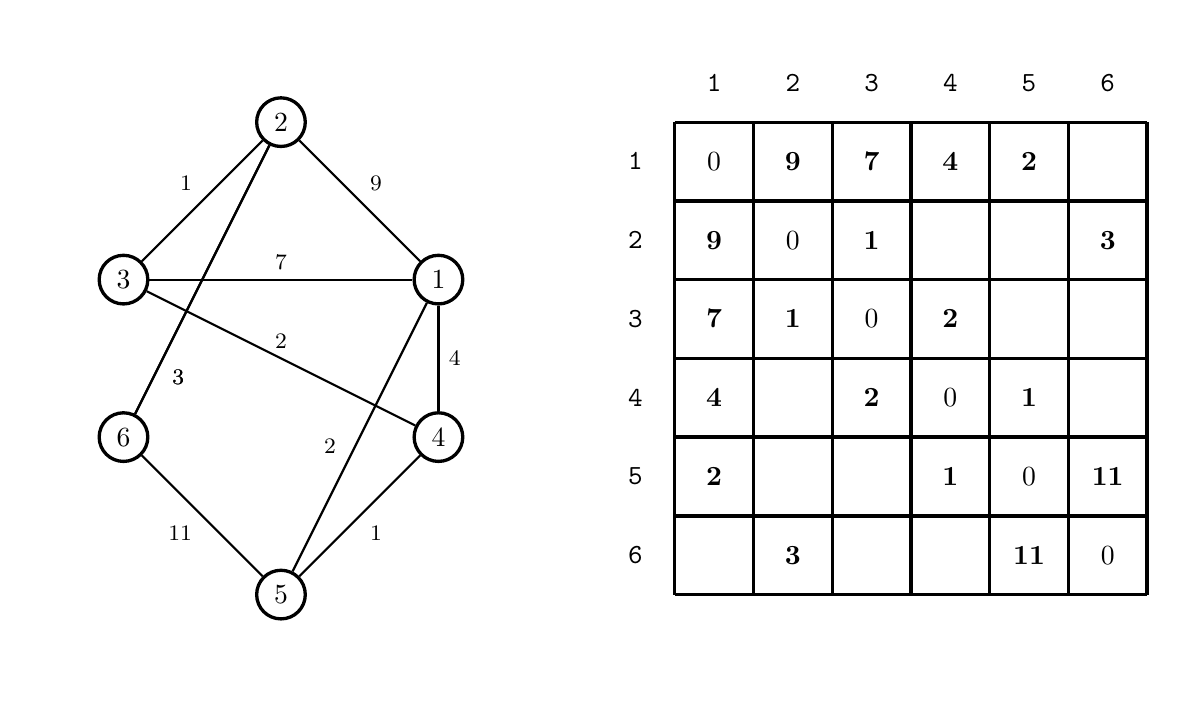
\begin{tikzpicture}
\node[draw,opacity=0] at (0, 0) {x};
\node[draw,opacity=0] at (14, 8) {x};

	\draw[very thick] (8.0, 1.0) grid  (14.0, 7.0);

	\node[] (x1) at (8.5, 7.5) { \bbtext{\tt 1} };

	\node[] (x2) at (9.5, 7.5) { \bbtext{\tt 2} };

	\node[] (x3) at (10.5, 7.5) { \bbtext{\tt 3} };

	\node[] (x4) at (11.5, 7.5) { \bbtext{\tt 4} };

	\node[] (x5) at (12.5, 7.5) { \bbtext{\tt 5} };

	\node[] (x6) at (13.5, 7.5) { \bbtext{\tt 6} };

	\node[] (y1) at (7.5, 6.5) { \bbtext{\tt 1} };

	\node[] (y2) at (7.5, 5.5) { \bbtext{\tt 2} };

	\node[] (y3) at (7.5, 4.5) { \bbtext{\tt 3} };

	\node[] (y4) at (7.5, 3.5) { \bbtext{\tt 4} };

	\node[] (y5) at (7.5, 2.5) { \bbtext{\tt 5} };

	\node[] (y6) at (7.5, 1.5) { \bbtext{\tt 6} };

	\node[very thick,draw,circle] (node1) at (5.0, 5.0) { \bbtext{1} };

	\node[very thick,draw,circle] (node2) at (3.0, 7.0) { \bbtext{2} };

	\node[very thick,draw,circle] (node3) at (1.0, 5.0) { \bbtext{3} };

	\node[very thick,draw,circle] (node4) at (5.0, 3.0) { \bbtext{4} };

	\node[very thick,draw,circle] (node5) at (3.0, 1.0) { \bbtext{5} };

	\node[very thick,draw,circle] (node6) at (1.0, 3.0) { \bbtext{6} };

	\draw[thick](node1) to node[above right] {\footnotesize \bbinfo{9}} (node2);

	\draw[thick](node1) to node[above] {\footnotesize \bbinfo{7}} (node3);

	\draw[thick](node1) to node[right] {\footnotesize \bbinfo{4}} (node4);

	\draw[thick](node1) to node[above left,pos=.6] {\footnotesize \bbinfo{2}} (node5);

	\draw[thick](node2) to node[above left] {\footnotesize \bbinfo{1}} (node3);

	\draw[thick](node2) to node[below right,pos=.8] {\footnotesize \bbinfo{3}} (node6);

	\draw[thick](node2) to node[below right,pos=.8] {\footnotesize \bbinfo{3}} (node6);

	\draw[thick](node3) to node[above] {\footnotesize \bbinfo{2}} (node4);

	\draw[thick](node4) to node[below right] {\footnotesize \bbinfo{1}} (node5);

	\draw[thick](node5) to node[below left] {\footnotesize \bbinfo{11}} (node6);


	\node[] (a11) at (8.5, 6.5) { $0$ };

	\node[] (a22) at (9.5, 5.5) { $0$ };

	\node[] (a33) at (10.5, 4.5) { $0$ };

	\node[] (a44) at (11.5, 3.5) { $0$ };

	\node[] (a55) at (12.5, 2.5) { $0$ };

	\node[] (a66) at (13.5, 1.5) { $0$ };



	\node[] (a12) at (9.5, 6.5) { $\mathbf{9}$ };

	\node[] (a21) at (8.5, 5.5) { $\mathbf{9}$ };

	\node[] (a13) at (10.5, 6.5) { $\mathbf{7}$ };

	\node[] (a31) at (8.5, 4.5) { $\mathbf{7}$ };

	\node[] (a14) at (11.5, 6.5) { $\mathbf{4}$ };

	\node[] (a41) at (8.5, 3.5) { $\mathbf{4}$ };

	\node[] (a15) at (12.5, 6.5) { $\mathbf{2}$ };

	\node[] (a51) at (8.5, 2.5) { $\mathbf{2}$ };

	\node[] (a23) at (10.5, 5.5) { $\mathbf{1}$ };

	\node[] (a32) at (9.5, 4.5) { $\mathbf{1}$ };

	\node[] (a26) at (13.5, 5.5) { $\mathbf{3}$ };

	\node[] (a62) at (9.5, 1.5) { $\mathbf{3}$ };

	\node[] (a34) at (11.5, 4.5) { $\mathbf{2}$ };

	\node[] (a43) at (10.5, 3.5) { $\mathbf{2}$ };

	\node[] (a45) at (12.5, 3.5) { $\mathbf{1}$ };

	\node[] (a54) at (11.5, 2.5) { $\mathbf{1}$ };

	\node[] (a56) at (13.5, 2.5) { $\mathbf{11}$ };

	\node[] (a65) at (12.5, 1.5) { $\mathbf{11}$ };

\end{tikzpicture}
\end{frame}
\begin{frame}[plain,t]
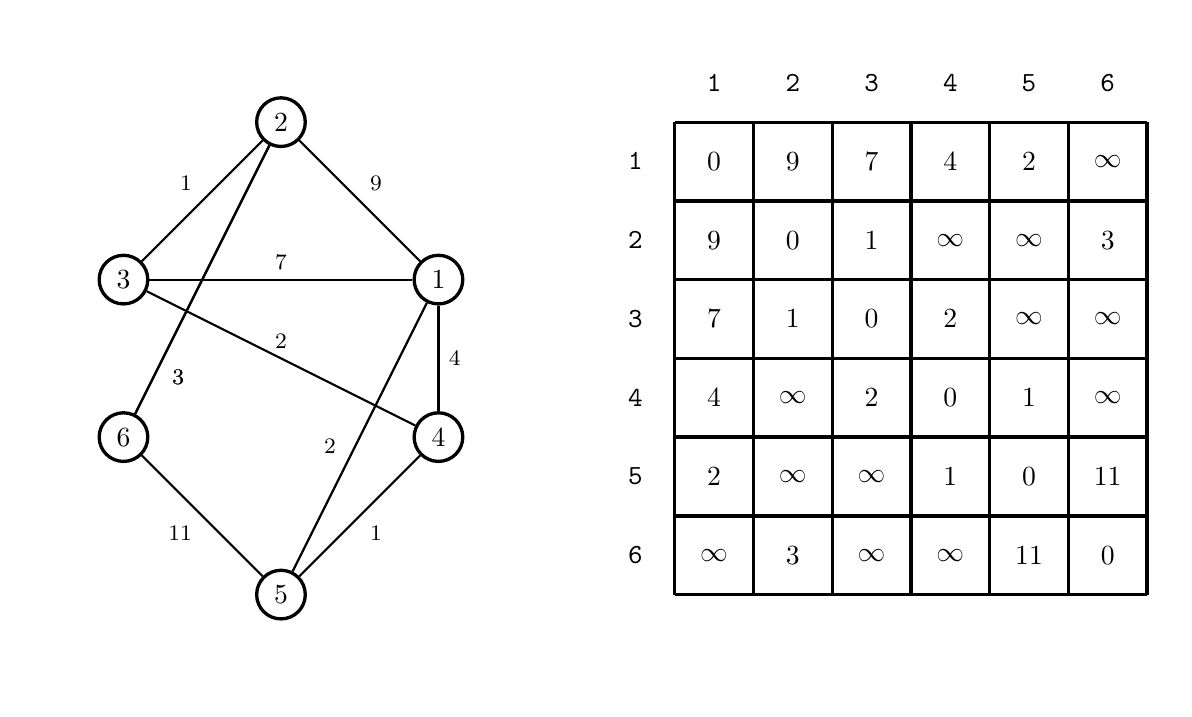
\begin{tikzpicture}
\node[draw,opacity=0] at (0, 0) {x};
\node[draw,opacity=0] at (14, 8) {x};

	\draw[very thick] (8.0, 1.0) grid  (14.0, 7.0);

	\node[] (x1) at (8.5, 7.5) { \bbtext{\tt 1} };

	\node[] (x2) at (9.5, 7.5) { \bbtext{\tt 2} };

	\node[] (x3) at (10.5, 7.5) { \bbtext{\tt 3} };

	\node[] (x4) at (11.5, 7.5) { \bbtext{\tt 4} };

	\node[] (x5) at (12.5, 7.5) { \bbtext{\tt 5} };

	\node[] (x6) at (13.5, 7.5) { \bbtext{\tt 6} };

	\node[] (y1) at (7.5, 6.5) { \bbtext{\tt 1} };

	\node[] (y2) at (7.5, 5.5) { \bbtext{\tt 2} };

	\node[] (y3) at (7.5, 4.5) { \bbtext{\tt 3} };

	\node[] (y4) at (7.5, 3.5) { \bbtext{\tt 4} };

	\node[] (y5) at (7.5, 2.5) { \bbtext{\tt 5} };

	\node[] (y6) at (7.5, 1.5) { \bbtext{\tt 6} };

	\node[very thick,draw,circle] (node1) at (5.0, 5.0) { \bbtext{1} };

	\node[very thick,draw,circle] (node2) at (3.0, 7.0) { \bbtext{2} };

	\node[very thick,draw,circle] (node3) at (1.0, 5.0) { \bbtext{3} };

	\node[very thick,draw,circle] (node4) at (5.0, 3.0) { \bbtext{4} };

	\node[very thick,draw,circle] (node5) at (3.0, 1.0) { \bbtext{5} };

	\node[very thick,draw,circle] (node6) at (1.0, 3.0) { \bbtext{6} };

	\draw[thick](node1) to node[above right] {\footnotesize \bbinfo{9}} (node2);

	\draw[thick](node1) to node[above] {\footnotesize \bbinfo{7}} (node3);

	\draw[thick](node1) to node[right] {\footnotesize \bbinfo{4}} (node4);

	\draw[thick](node1) to node[above left,pos=.6] {\footnotesize \bbinfo{2}} (node5);

	\draw[thick](node2) to node[above left] {\footnotesize \bbinfo{1}} (node3);

	\draw[thick](node2) to node[below right,pos=.8] {\footnotesize \bbinfo{3}} (node6);

	\draw[thick](node2) to node[below right,pos=.8] {\footnotesize \bbinfo{3}} (node6);

	\draw[thick](node3) to node[above] {\footnotesize \bbinfo{2}} (node4);

	\draw[thick](node4) to node[below right] {\footnotesize \bbinfo{1}} (node5);

	\draw[thick](node5) to node[below left] {\footnotesize \bbinfo{11}} (node6);


	\node[] (a11) at (8.5, 6.5) { $0$ };

	\node[] (a22) at (9.5, 5.5) { $0$ };

	\node[] (a33) at (10.5, 4.5) { $0$ };

	\node[] (a44) at (11.5, 3.5) { $0$ };

	\node[] (a55) at (12.5, 2.5) { $0$ };

	\node[] (a66) at (13.5, 1.5) { $0$ };



	\node[] (a12) at (9.5, 6.5) { $9$ };

	\node[] (a21) at (8.5, 5.5) { $9$ };

	\node[] (a13) at (10.5, 6.5) { $7$ };

	\node[] (a31) at (8.5, 4.5) { $7$ };

	\node[] (a14) at (11.5, 6.5) { $4$ };

	\node[] (a41) at (8.5, 3.5) { $4$ };

	\node[] (a15) at (12.5, 6.5) { $2$ };

	\node[] (a51) at (8.5, 2.5) { $2$ };

	\node[] (a23) at (10.5, 5.5) { $1$ };

	\node[] (a32) at (9.5, 4.5) { $1$ };

	\node[] (a26) at (13.5, 5.5) { $3$ };

	\node[] (a62) at (9.5, 1.5) { $3$ };

	\node[] (a34) at (11.5, 4.5) { $2$ };

	\node[] (a43) at (10.5, 3.5) { $2$ };

	\node[] (a45) at (12.5, 3.5) { $1$ };

	\node[] (a54) at (11.5, 2.5) { $1$ };

	\node[] (a56) at (13.5, 2.5) { $11$ };

	\node[] (a65) at (12.5, 1.5) { $11$ };



	\node[] (a16) at (13.5, 6.5) { $\mathbf{\infty}$ };

	\node[] (a24) at (11.5, 5.5) { $\mathbf{\infty}$ };

	\node[] (a25) at (12.5, 5.5) { $\mathbf{\infty}$ };

	\node[] (a35) at (12.5, 4.5) { $\mathbf{\infty}$ };

	\node[] (a36) at (13.5, 4.5) { $\mathbf{\infty}$ };

	\node[] (a42) at (9.5, 3.5) { $\mathbf{\infty}$ };

	\node[] (a46) at (13.5, 3.5) { $\mathbf{\infty}$ };

	\node[] (a52) at (9.5, 2.5) { $\mathbf{\infty}$ };

	\node[] (a53) at (10.5, 2.5) { $\mathbf{\infty}$ };

	\node[] (a61) at (8.5, 1.5) { $\mathbf{\infty}$ };

	\node[] (a63) at (10.5, 1.5) { $\mathbf{\infty}$ };

	\node[] (a64) at (11.5, 1.5) { $\mathbf{\infty}$ };

\end{tikzpicture}
\end{frame}
\begin{frame}[plain,t]
\begin{tikzpicture}
\node[draw,opacity=0] at (0, 0) {x};
\node[draw,opacity=0] at (14, 8) {x};

	\draw[very thick] (8.0, 1.0) grid  (14.0, 7.0);

	\node[] (x1) at (8.5, 7.5) { \bbtext{\tt 1} };

	\node[] (x2) at (9.5, 7.5) { \bbtext{\tt 2} };

	\node[] (x3) at (10.5, 7.5) { \bbtext{\tt 3} };

	\node[] (x4) at (11.5, 7.5) { \bbtext{\tt 4} };

	\node[] (x5) at (12.5, 7.5) { \bbtext{\tt 5} };

	\node[] (x6) at (13.5, 7.5) { \bbtext{\tt 6} };

	\node[] (y1) at (7.5, 6.5) { \bbtext{\tt 1} };

	\node[] (y2) at (7.5, 5.5) { \bbtext{\tt 2} };

	\node[] (y3) at (7.5, 4.5) { \bbtext{\tt 3} };

	\node[] (y4) at (7.5, 3.5) { \bbtext{\tt 4} };

	\node[] (y5) at (7.5, 2.5) { \bbtext{\tt 5} };

	\node[] (y6) at (7.5, 1.5) { \bbtext{\tt 6} };

	\node[very thick,draw,circle,fill=BBCyan] (node1) at (5.0, 5.0) { \bbtext{1} };

	\node[very thick,draw,circle] (node2) at (3.0, 7.0) { \bbtext{2} };

	\node[very thick,draw,circle] (node3) at (1.0, 5.0) { \bbtext{3} };

	\node[very thick,draw,circle] (node4) at (5.0, 3.0) { \bbtext{4} };

	\node[very thick,draw,circle] (node5) at (3.0, 1.0) { \bbtext{5} };

	\node[very thick,draw,circle] (node6) at (1.0, 3.0) { \bbtext{6} };

	\draw[thick](node1) to node[above right] {\footnotesize \bbinfo{9}} (node2);

	\draw[thick](node1) to node[above] {\footnotesize \bbinfo{7}} (node3);

	\draw[thick](node1) to node[right] {\footnotesize \bbinfo{4}} (node4);

	\draw[thick](node1) to node[above left,pos=.6] {\footnotesize \bbinfo{2}} (node5);

	\draw[thick](node2) to node[above left] {\footnotesize \bbinfo{1}} (node3);

	\draw[thick](node2) to node[below right,pos=.8] {\footnotesize \bbinfo{3}} (node6);

	\draw[thick](node2) to node[below right,pos=.8] {\footnotesize \bbinfo{3}} (node6);

	\draw[thick](node3) to node[above] {\footnotesize \bbinfo{2}} (node4);

	\draw[thick](node4) to node[below right] {\footnotesize \bbinfo{1}} (node5);

	\draw[thick](node5) to node[below left] {\footnotesize \bbinfo{11}} (node6);


	\node[] (a11) at (8.5, 6.5) { $0$ };

	\node[] (a22) at (9.5, 5.5) { $0$ };

	\node[] (a33) at (10.5, 4.5) { $0$ };

	\node[] (a44) at (11.5, 3.5) { $0$ };

	\node[] (a55) at (12.5, 2.5) { $0$ };

	\node[] (a66) at (13.5, 1.5) { $0$ };



	\node[] (a12) at (9.5, 6.5) { $9$ };

	\node[] (a21) at (8.5, 5.5) { $9$ };

	\node[] (a13) at (10.5, 6.5) { $7$ };

	\node[] (a31) at (8.5, 4.5) { $7$ };

	\node[] (a14) at (11.5, 6.5) { $4$ };

	\node[] (a41) at (8.5, 3.5) { $4$ };

	\node[] (a15) at (12.5, 6.5) { $2$ };

	\node[] (a51) at (8.5, 2.5) { $2$ };

	\node[] (a23) at (10.5, 5.5) { $1$ };

	\node[] (a32) at (9.5, 4.5) { $1$ };

	\node[] (a26) at (13.5, 5.5) { $3$ };

	\node[] (a62) at (9.5, 1.5) { $3$ };

	\node[] (a34) at (11.5, 4.5) { $2$ };

	\node[] (a43) at (10.5, 3.5) { $2$ };

	\node[] (a45) at (12.5, 3.5) { $1$ };

	\node[] (a54) at (11.5, 2.5) { $1$ };

	\node[] (a56) at (13.5, 2.5) { $11$ };

	\node[] (a65) at (12.5, 1.5) { $11$ };



	\node[] (a16) at (13.5, 6.5) { $\mathbf{\infty}$ };

	\node[] (a24) at (11.5, 5.5) { $\mathbf{13}$ };

	\node[] (a25) at (12.5, 5.5) { $\mathbf{11}$ };

	\node[] (a35) at (12.5, 4.5) { $\mathbf{9}$ };

	\node[] (a36) at (13.5, 4.5) { $\mathbf{\infty}$ };

	\node[] (a42) at (9.5, 3.5) { $\mathbf{13}$ };

	\node[] (a46) at (13.5, 3.5) { $\mathbf{\infty}$ };

	\node[] (a52) at (9.5, 2.5) { $\mathbf{11}$ };

	\node[] (a53) at (10.5, 2.5) { $\mathbf{9}$ };

	\node[] (a61) at (8.5, 1.5) { $\mathbf{\infty}$ };

	\node[] (a63) at (10.5, 1.5) { $\mathbf{\infty}$ };

	\node[] (a64) at (11.5, 1.5) { $\mathbf{\infty}$ };




\end{tikzpicture}
\end{frame}
\begin{frame}[plain,t]
\begin{tikzpicture}
\node[draw,opacity=0] at (0, 0) {x};
\node[draw,opacity=0] at (14, 8) {x};

	\draw[very thick] (8.0, 1.0) grid  (14.0, 7.0);

	\node[] (x1) at (8.5, 7.5) { \bbtext{\tt 1} };

	\node[] (x2) at (9.5, 7.5) { \bbtext{\tt 2} };

	\node[] (x3) at (10.5, 7.5) { \bbtext{\tt 3} };

	\node[] (x4) at (11.5, 7.5) { \bbtext{\tt 4} };

	\node[] (x5) at (12.5, 7.5) { \bbtext{\tt 5} };

	\node[] (x6) at (13.5, 7.5) { \bbtext{\tt 6} };

	\node[] (y1) at (7.5, 6.5) { \bbtext{\tt 1} };

	\node[] (y2) at (7.5, 5.5) { \bbtext{\tt 2} };

	\node[] (y3) at (7.5, 4.5) { \bbtext{\tt 3} };

	\node[] (y4) at (7.5, 3.5) { \bbtext{\tt 4} };

	\node[] (y5) at (7.5, 2.5) { \bbtext{\tt 5} };

	\node[] (y6) at (7.5, 1.5) { \bbtext{\tt 6} };

	\node[very thick,draw,circle,fill=BBGreen] (node1) at (5.0, 5.0) { \bbtext{1} };

	\node[very thick,draw,circle,fill=BBCyan] (node2) at (3.0, 7.0) { \bbtext{2} };

	\node[very thick,draw,circle] (node3) at (1.0, 5.0) { \bbtext{3} };

	\node[very thick,draw,circle] (node4) at (5.0, 3.0) { \bbtext{4} };

	\node[very thick,draw,circle] (node5) at (3.0, 1.0) { \bbtext{5} };

	\node[very thick,draw,circle] (node6) at (1.0, 3.0) { \bbtext{6} };

	\draw[thick](node1) to node[above right] {\footnotesize \bbinfo{9}} (node2);

	\draw[thick](node1) to node[above] {\footnotesize \bbinfo{7}} (node3);

	\draw[thick](node1) to node[right] {\footnotesize \bbinfo{4}} (node4);

	\draw[thick](node1) to node[above left,pos=.6] {\footnotesize \bbinfo{2}} (node5);

	\draw[thick](node2) to node[above left] {\footnotesize \bbinfo{1}} (node3);

	\draw[thick](node2) to node[below right,pos=.8] {\footnotesize \bbinfo{3}} (node6);

	\draw[thick](node2) to node[below right,pos=.8] {\footnotesize \bbinfo{3}} (node6);

	\draw[thick](node3) to node[above] {\footnotesize \bbinfo{2}} (node4);

	\draw[thick](node4) to node[below right] {\footnotesize \bbinfo{1}} (node5);

	\draw[thick](node5) to node[below left] {\footnotesize \bbinfo{11}} (node6);


	\node[] (a11) at (8.5, 6.5) { $0$ };

	\node[] (a22) at (9.5, 5.5) { $0$ };

	\node[] (a33) at (10.5, 4.5) { $0$ };

	\node[] (a44) at (11.5, 3.5) { $0$ };

	\node[] (a55) at (12.5, 2.5) { $0$ };

	\node[] (a66) at (13.5, 1.5) { $0$ };



	\node[] (a12) at (9.5, 6.5) { $9$ };

	\node[] (a21) at (8.5, 5.5) { $9$ };

	\node[] (a13) at (10.5, 6.5) { $7$ };

	\node[] (a31) at (8.5, 4.5) { $7$ };

	\node[] (a14) at (11.5, 6.5) { $4$ };

	\node[] (a41) at (8.5, 3.5) { $4$ };

	\node[] (a15) at (12.5, 6.5) { $2$ };

	\node[] (a51) at (8.5, 2.5) { $2$ };

	\node[] (a23) at (10.5, 5.5) { $1$ };

	\node[] (a32) at (9.5, 4.5) { $1$ };

	\node[] (a26) at (13.5, 5.5) { $3$ };

	\node[] (a62) at (9.5, 1.5) { $3$ };

	\node[] (a34) at (11.5, 4.5) { $2$ };

	\node[] (a43) at (10.5, 3.5) { $2$ };

	\node[] (a45) at (12.5, 3.5) { $1$ };

	\node[] (a54) at (11.5, 2.5) { $1$ };

	\node[] (a56) at (13.5, 2.5) { $11$ };

	\node[] (a65) at (12.5, 1.5) { $11$ };



	\node[] (a16) at (13.5, 6.5) { $\mathbf{12}$ };

	\node[] (a24) at (11.5, 5.5) { ${13}$ };

	\node[] (a25) at (12.5, 5.5) { ${11}$ };

	\node[] (a35) at (12.5, 4.5) { ${9}$ };

	\node[] (a36) at (13.5, 4.5) { $\mathbf{4}$ };

	\node[] (a42) at (9.5, 3.5) { ${13}$ };

	\node[] (a46) at (13.5, 3.5) { $\mathbf{16}$ };

	\node[] (a52) at (9.5, 2.5) { ${11}$ };

	\node[] (a53) at (10.5, 2.5) { ${9}$ };

	\node[] (a61) at (8.5, 1.5) { $\mathbf{12}$ };

	\node[] (a63) at (10.5, 1.5) { $\mathbf{4}$ };

	\node[] (a64) at (11.5, 1.5) { $\mathbf{16}$ };







\end{tikzpicture}
\end{frame}
\begin{frame}[plain,t]
\begin{tikzpicture}
\node[draw,opacity=0] at (0, 0) {x};
\node[draw,opacity=0] at (14, 8) {x};

	\draw[very thick] (8.0, 1.0) grid  (14.0, 7.0);

	\node[] (x1) at (8.5, 7.5) { \bbtext{\tt 1} };

	\node[] (x2) at (9.5, 7.5) { \bbtext{\tt 2} };

	\node[] (x3) at (10.5, 7.5) { \bbtext{\tt 3} };

	\node[] (x4) at (11.5, 7.5) { \bbtext{\tt 4} };

	\node[] (x5) at (12.5, 7.5) { \bbtext{\tt 5} };

	\node[] (x6) at (13.5, 7.5) { \bbtext{\tt 6} };

	\node[] (y1) at (7.5, 6.5) { \bbtext{\tt 1} };

	\node[] (y2) at (7.5, 5.5) { \bbtext{\tt 2} };

	\node[] (y3) at (7.5, 4.5) { \bbtext{\tt 3} };

	\node[] (y4) at (7.5, 3.5) { \bbtext{\tt 4} };

	\node[] (y5) at (7.5, 2.5) { \bbtext{\tt 5} };

	\node[] (y6) at (7.5, 1.5) { \bbtext{\tt 6} };

	\node[very thick,draw,circle,fill=BBGreen] (node1) at (5.0, 5.0) { \bbtext{1} };

	\node[very thick,draw,circle,fill=BBGreen] (node2) at (3.0, 7.0) { \bbtext{2} };

	\node[very thick,draw,circle,fill=BBCyan] (node3) at (1.0, 5.0) { \bbtext{3} };

	\node[very thick,draw,circle] (node4) at (5.0, 3.0) { \bbtext{4} };

	\node[very thick,draw,circle] (node5) at (3.0, 1.0) { \bbtext{5} };

	\node[very thick,draw,circle] (node6) at (1.0, 3.0) { \bbtext{6} };

	\draw[thick](node1) to node[above right] {\footnotesize \bbinfo{9}} (node2);

	\draw[thick](node1) to node[above] {\footnotesize \bbinfo{7}} (node3);

	\draw[thick](node1) to node[right] {\footnotesize \bbinfo{4}} (node4);

	\draw[thick](node1) to node[above left,pos=.6] {\footnotesize \bbinfo{2}} (node5);

	\draw[thick](node2) to node[above left] {\footnotesize \bbinfo{1}} (node3);

	\draw[thick](node2) to node[below right,pos=.8] {\footnotesize \bbinfo{3}} (node6);

	\draw[thick](node2) to node[below right,pos=.8] {\footnotesize \bbinfo{3}} (node6);

	\draw[thick](node3) to node[above] {\footnotesize \bbinfo{2}} (node4);

	\draw[thick](node4) to node[below right] {\footnotesize \bbinfo{1}} (node5);

	\draw[thick](node5) to node[below left] {\footnotesize \bbinfo{11}} (node6);


	\node[] (a11) at (8.5, 6.5) { $0$ };

	\node[] (a22) at (9.5, 5.5) { $0$ };

	\node[] (a33) at (10.5, 4.5) { $0$ };

	\node[] (a44) at (11.5, 3.5) { $0$ };

	\node[] (a55) at (12.5, 2.5) { $0$ };

	\node[] (a66) at (13.5, 1.5) { $0$ };



	\node[] (a12) at (9.5, 6.5) { $\mathbf{8}$ };

	\node[] (a21) at (8.5, 5.5) { $\mathbf{8}$ };

	\node[] (a13) at (10.5, 6.5) { $7$ };

	\node[] (a31) at (8.5, 4.5) { $7$ };

	\node[] (a14) at (11.5, 6.5) { $4$ };

	\node[] (a41) at (8.5, 3.5) { $4$ };

	\node[] (a15) at (12.5, 6.5) { $2$ };

	\node[] (a51) at (8.5, 2.5) { $2$ };

	\node[] (a23) at (10.5, 5.5) { $1$ };

	\node[] (a32) at (9.5, 4.5) { $1$ };

	\node[] (a26) at (13.5, 5.5) { $3$ };

	\node[] (a62) at (9.5, 1.5) { $3$ };

	\node[] (a34) at (11.5, 4.5) { $2$ };

	\node[] (a43) at (10.5, 3.5) { $2$ };

	\node[] (a45) at (12.5, 3.5) { $1$ };

	\node[] (a54) at (11.5, 2.5) { $1$ };

	\node[] (a56) at (13.5, 2.5) { $11$ };

	\node[] (a65) at (12.5, 1.5) { $11$ };



	\node[] (a16) at (13.5, 6.5) { $\mathbf{11}$ };

	\node[] (a24) at (11.5, 5.5) { $\mathbf{3}$ };

	\node[] (a25) at (12.5, 5.5) { $\mathbf{10}$ };

	\node[] (a35) at (12.5, 4.5) { ${9}$ };

	\node[] (a36) at (13.5, 4.5) { ${4}$ };

	\node[] (a42) at (9.5, 3.5) { $\mathbf{3}$ };

	\node[] (a46) at (13.5, 3.5) { $\mathbf{6}$ };

	\node[] (a52) at (9.5, 2.5) { $\mathbf{10}$ };

	\node[] (a53) at (10.5, 2.5) { ${9}$ };

	\node[] (a61) at (8.5, 1.5) { $\mathbf{11}$ };

	\node[] (a63) at (10.5, 1.5) { ${4}$ };

	\node[] (a64) at (11.5, 1.5) { $\mathbf{6}$ };












\end{tikzpicture}
\end{frame}
\begin{frame}[plain,t]
\begin{tikzpicture}
\node[draw,opacity=0] at (0, 0) {x};
\node[draw,opacity=0] at (14, 8) {x};

	\draw[very thick] (8.0, 1.0) grid  (14.0, 7.0);

	\node[] (x1) at (8.5, 7.5) { \bbtext{\tt 1} };

	\node[] (x2) at (9.5, 7.5) { \bbtext{\tt 2} };

	\node[] (x3) at (10.5, 7.5) { \bbtext{\tt 3} };

	\node[] (x4) at (11.5, 7.5) { \bbtext{\tt 4} };

	\node[] (x5) at (12.5, 7.5) { \bbtext{\tt 5} };

	\node[] (x6) at (13.5, 7.5) { \bbtext{\tt 6} };

	\node[] (y1) at (7.5, 6.5) { \bbtext{\tt 1} };

	\node[] (y2) at (7.5, 5.5) { \bbtext{\tt 2} };

	\node[] (y3) at (7.5, 4.5) { \bbtext{\tt 3} };

	\node[] (y4) at (7.5, 3.5) { \bbtext{\tt 4} };

	\node[] (y5) at (7.5, 2.5) { \bbtext{\tt 5} };

	\node[] (y6) at (7.5, 1.5) { \bbtext{\tt 6} };

	\node[very thick,draw,circle,fill=BBGreen] (node1) at (5.0, 5.0) { \bbtext{1} };

	\node[very thick,draw,circle,fill=BBGreen] (node2) at (3.0, 7.0) { \bbtext{2} };

	\node[very thick,draw,circle,fill=BBGreen] (node3) at (1.0, 5.0) { \bbtext{3} };

	\node[very thick,draw,circle,fill=BBCyan] (node4) at (5.0, 3.0) { \bbtext{4} };

	\node[very thick,draw,circle] (node5) at (3.0, 1.0) { \bbtext{5} };

	\node[very thick,draw,circle] (node6) at (1.0, 3.0) { \bbtext{6} };

	\draw[thick](node1) to node[above right] {\footnotesize \bbinfo{9}} (node2);

	\draw[thick](node1) to node[above] {\footnotesize \bbinfo{7}} (node3);

	\draw[thick](node1) to node[right] {\footnotesize \bbinfo{4}} (node4);

	\draw[thick](node1) to node[above left,pos=.6] {\footnotesize \bbinfo{2}} (node5);

	\draw[thick](node2) to node[above left] {\footnotesize \bbinfo{1}} (node3);

	\draw[thick](node2) to node[below right,pos=.8] {\footnotesize \bbinfo{3}} (node6);

	\draw[thick](node2) to node[below right,pos=.8] {\footnotesize \bbinfo{3}} (node6);

	\draw[thick](node3) to node[above] {\footnotesize \bbinfo{2}} (node4);

	\draw[thick](node4) to node[below right] {\footnotesize \bbinfo{1}} (node5);

	\draw[thick](node5) to node[below left] {\footnotesize \bbinfo{11}} (node6);


	\node[] (a11) at (8.5, 6.5) { $0$ };

	\node[] (a22) at (9.5, 5.5) { $0$ };

	\node[] (a33) at (10.5, 4.5) { $0$ };

	\node[] (a44) at (11.5, 3.5) { $0$ };

	\node[] (a55) at (12.5, 2.5) { $0$ };

	\node[] (a66) at (13.5, 1.5) { $0$ };



	\node[] (a12) at (9.5, 6.5) { $\mathbf{7}$ };

	\node[] (a21) at (8.5, 5.5) { $\mathbf{7}$ };

	\node[] (a13) at (10.5, 6.5) { $\mathbf{6}$ };

	\node[] (a31) at (8.5, 4.5) { $\mathbf{6}$ };

	\node[] (a14) at (11.5, 6.5) { $4$ };

	\node[] (a41) at (8.5, 3.5) { $4$ };

	\node[] (a15) at (12.5, 6.5) { $2$ };

	\node[] (a51) at (8.5, 2.5) { $2$ };

	\node[] (a23) at (10.5, 5.5) { $1$ };

	\node[] (a32) at (9.5, 4.5) { $1$ };

	\node[] (a26) at (13.5, 5.5) { $3$ };

	\node[] (a62) at (9.5, 1.5) { $3$ };

	\node[] (a34) at (11.5, 4.5) { $2$ };

	\node[] (a43) at (10.5, 3.5) { $2$ };

	\node[] (a45) at (12.5, 3.5) { $1$ };

	\node[] (a54) at (11.5, 2.5) { $1$ };

	\node[] (a56) at (13.5, 2.5) { $\mathbf{7}$ };

	\node[] (a65) at (12.5, 1.5) { $\mathbf{7}$ };



	\node[] (a16) at (13.5, 6.5) { $\mathbf{10}$ };

	\node[] (a24) at (11.5, 5.5) { ${3}$ };

	\node[] (a25) at (12.5, 5.5) { $\mathbf{4}$ };

	\node[] (a35) at (12.5, 4.5) { $\mathbf{3}$ };

	\node[] (a36) at (13.5, 4.5) { ${4}$ };

	\node[] (a42) at (9.5, 3.5) { ${3}$ };

	\node[] (a46) at (13.5, 3.5) { ${6}$ };

	\node[] (a52) at (9.5, 2.5) { $\mathbf{4}$ };

	\node[] (a53) at (10.5, 2.5) { $\mathbf{3}$ };

	\node[] (a61) at (8.5, 1.5) { $\mathbf{10}$ };

	\node[] (a63) at (10.5, 1.5) { ${4}$ };

	\node[] (a64) at (11.5, 1.5) { ${6}$ };
















\end{tikzpicture}
\end{frame}
\begin{frame}[plain,t]
\begin{tikzpicture}
\node[draw,opacity=0] at (0, 0) {x};
\node[draw,opacity=0] at (14, 8) {x};

	\draw[very thick] (8.0, 1.0) grid  (14.0, 7.0);

	\node[] (x1) at (8.5, 7.5) { \bbtext{\tt 1} };

	\node[] (x2) at (9.5, 7.5) { \bbtext{\tt 2} };

	\node[] (x3) at (10.5, 7.5) { \bbtext{\tt 3} };

	\node[] (x4) at (11.5, 7.5) { \bbtext{\tt 4} };

	\node[] (x5) at (12.5, 7.5) { \bbtext{\tt 5} };

	\node[] (x6) at (13.5, 7.5) { \bbtext{\tt 6} };

	\node[] (y1) at (7.5, 6.5) { \bbtext{\tt 1} };

	\node[] (y2) at (7.5, 5.5) { \bbtext{\tt 2} };

	\node[] (y3) at (7.5, 4.5) { \bbtext{\tt 3} };

	\node[] (y4) at (7.5, 3.5) { \bbtext{\tt 4} };

	\node[] (y5) at (7.5, 2.5) { \bbtext{\tt 5} };

	\node[] (y6) at (7.5, 1.5) { \bbtext{\tt 6} };

	\node[very thick,draw,circle,fill=BBGreen] (node1) at (5.0, 5.0) { \bbtext{1} };

	\node[very thick,draw,circle,fill=BBGreen] (node2) at (3.0, 7.0) { \bbtext{2} };

	\node[very thick,draw,circle,fill=BBGreen] (node3) at (1.0, 5.0) { \bbtext{3} };

	\node[very thick,draw,circle,fill=BBGreen] (node4) at (5.0, 3.0) { \bbtext{4} };

	\node[very thick,draw,circle,fill=BBCyan] (node5) at (3.0, 1.0) { \bbtext{5} };

	\node[very thick,draw,circle] (node6) at (1.0, 3.0) { \bbtext{6} };

	\draw[thick](node1) to node[above right] {\footnotesize \bbinfo{9}} (node2);

	\draw[thick](node1) to node[above] {\footnotesize \bbinfo{7}} (node3);

	\draw[thick](node1) to node[right] {\footnotesize \bbinfo{4}} (node4);

	\draw[thick](node1) to node[above left,pos=.6] {\footnotesize \bbinfo{2}} (node5);

	\draw[thick](node2) to node[above left] {\footnotesize \bbinfo{1}} (node3);

	\draw[thick](node2) to node[below right,pos=.8] {\footnotesize \bbinfo{3}} (node6);

	\draw[thick](node2) to node[below right,pos=.8] {\footnotesize \bbinfo{3}} (node6);

	\draw[thick](node3) to node[above] {\footnotesize \bbinfo{2}} (node4);

	\draw[thick](node4) to node[below right] {\footnotesize \bbinfo{1}} (node5);

	\draw[thick](node5) to node[below left] {\footnotesize \bbinfo{11}} (node6);


	\node[] (a11) at (8.5, 6.5) { $0$ };

	\node[] (a22) at (9.5, 5.5) { $0$ };

	\node[] (a33) at (10.5, 4.5) { $0$ };

	\node[] (a44) at (11.5, 3.5) { $0$ };

	\node[] (a55) at (12.5, 2.5) { $0$ };

	\node[] (a66) at (13.5, 1.5) { $0$ };



	\node[] (a12) at (9.5, 6.5) { $\mathbf{6}$ };

	\node[] (a21) at (8.5, 5.5) { $\mathbf{6}$ };

	\node[] (a13) at (10.5, 6.5) { $\mathbf{5}$ };

	\node[] (a31) at (8.5, 4.5) { $\mathbf{5}$ };

	\node[] (a14) at (11.5, 6.5) { $\mathbf{3}$ };

	\node[] (a41) at (8.5, 3.5) { $\mathbf{3}$ };

	\node[] (a15) at (12.5, 6.5) { $2$ };

	\node[] (a51) at (8.5, 2.5) { $2$ };

	\node[] (a23) at (10.5, 5.5) { $1$ };

	\node[] (a32) at (9.5, 4.5) { $1$ };

	\node[] (a26) at (13.5, 5.5) { $3$ };

	\node[] (a62) at (9.5, 1.5) { $3$ };

	\node[] (a34) at (11.5, 4.5) { $2$ };

	\node[] (a43) at (10.5, 3.5) { $2$ };

	\node[] (a45) at (12.5, 3.5) { $1$ };

	\node[] (a54) at (11.5, 2.5) { $1$ };

	\node[] (a56) at (13.5, 2.5) { ${7}$ };

	\node[] (a65) at (12.5, 1.5) { ${7}$ };



	\node[] (a16) at (13.5, 6.5) { $\mathbf{9}$ };

	\node[] (a24) at (11.5, 5.5) { ${3}$ };

	\node[] (a25) at (12.5, 5.5) { ${4}$ };

	\node[] (a35) at (12.5, 4.5) { ${3}$ };

	\node[] (a36) at (13.5, 4.5) { ${4}$ };

	\node[] (a42) at (9.5, 3.5) { ${3}$ };

	\node[] (a46) at (13.5, 3.5) { ${6}$ };

	\node[] (a52) at (9.5, 2.5) { ${4}$ };

	\node[] (a53) at (10.5, 2.5) { ${3}$ };

	\node[] (a61) at (8.5, 1.5) { $\mathbf{9}$ };

	\node[] (a63) at (10.5, 1.5) { ${4}$ };

	\node[] (a64) at (11.5, 1.5) { ${6}$ };




















\end{tikzpicture}
\end{frame}
\begin{frame}[plain,t]
\begin{tikzpicture}
\node[draw,opacity=0] at (0, 0) {x};
\node[draw,opacity=0] at (14, 8) {x};

	\draw[very thick] (8.0, 1.0) grid  (14.0, 7.0);

	\node[] (x1) at (8.5, 7.5) { \bbtext{\tt 1} };

	\node[] (x2) at (9.5, 7.5) { \bbtext{\tt 2} };

	\node[] (x3) at (10.5, 7.5) { \bbtext{\tt 3} };

	\node[] (x4) at (11.5, 7.5) { \bbtext{\tt 4} };

	\node[] (x5) at (12.5, 7.5) { \bbtext{\tt 5} };

	\node[] (x6) at (13.5, 7.5) { \bbtext{\tt 6} };

	\node[] (y1) at (7.5, 6.5) { \bbtext{\tt 1} };

	\node[] (y2) at (7.5, 5.5) { \bbtext{\tt 2} };

	\node[] (y3) at (7.5, 4.5) { \bbtext{\tt 3} };

	\node[] (y4) at (7.5, 3.5) { \bbtext{\tt 4} };

	\node[] (y5) at (7.5, 2.5) { \bbtext{\tt 5} };

	\node[] (y6) at (7.5, 1.5) { \bbtext{\tt 6} };

	\node[very thick,draw,circle,fill=BBGreen] (node1) at (5.0, 5.0) { \bbtext{1} };

	\node[very thick,draw,circle,fill=BBGreen] (node2) at (3.0, 7.0) { \bbtext{2} };

	\node[very thick,draw,circle,fill=BBGreen] (node3) at (1.0, 5.0) { \bbtext{3} };

	\node[very thick,draw,circle,fill=BBGreen] (node4) at (5.0, 3.0) { \bbtext{4} };

	\node[very thick,draw,circle,fill=BBGreen] (node5) at (3.0, 1.0) { \bbtext{5} };

	\node[very thick,draw,circle,fill=BBCyan] (node6) at (1.0, 3.0) { \bbtext{6} };

	\draw[thick](node1) to node[above right] {\footnotesize \bbinfo{9}} (node2);

	\draw[thick](node1) to node[above] {\footnotesize \bbinfo{7}} (node3);

	\draw[thick](node1) to node[right] {\footnotesize \bbinfo{4}} (node4);

	\draw[thick](node1) to node[above left,pos=.6] {\footnotesize \bbinfo{2}} (node5);

	\draw[thick](node2) to node[above left] {\footnotesize \bbinfo{1}} (node3);

	\draw[thick](node2) to node[below right,pos=.8] {\footnotesize \bbinfo{3}} (node6);

	\draw[thick](node2) to node[below right,pos=.8] {\footnotesize \bbinfo{3}} (node6);

	\draw[thick](node3) to node[above] {\footnotesize \bbinfo{2}} (node4);

	\draw[thick](node4) to node[below right] {\footnotesize \bbinfo{1}} (node5);

	\draw[thick](node5) to node[below left] {\footnotesize \bbinfo{11}} (node6);


	\node[] (a11) at (8.5, 6.5) { $0$ };

	\node[] (a22) at (9.5, 5.5) { $0$ };

	\node[] (a33) at (10.5, 4.5) { $0$ };

	\node[] (a44) at (11.5, 3.5) { $0$ };

	\node[] (a55) at (12.5, 2.5) { $0$ };

	\node[] (a66) at (13.5, 1.5) { $0$ };



	\node[] (a12) at (9.5, 6.5) { ${6}$ };

	\node[] (a21) at (8.5, 5.5) { ${6}$ };

	\node[] (a13) at (10.5, 6.5) { ${5}$ };

	\node[] (a31) at (8.5, 4.5) { ${5}$ };

	\node[] (a14) at (11.5, 6.5) { ${3}$ };

	\node[] (a41) at (8.5, 3.5) { ${3}$ };

	\node[] (a15) at (12.5, 6.5) { $2$ };

	\node[] (a51) at (8.5, 2.5) { $2$ };

	\node[] (a23) at (10.5, 5.5) { $1$ };

	\node[] (a32) at (9.5, 4.5) { $1$ };

	\node[] (a26) at (13.5, 5.5) { $3$ };

	\node[] (a62) at (9.5, 1.5) { $3$ };

	\node[] (a34) at (11.5, 4.5) { $2$ };

	\node[] (a43) at (10.5, 3.5) { $2$ };

	\node[] (a45) at (12.5, 3.5) { $1$ };

	\node[] (a54) at (11.5, 2.5) { $1$ };

	\node[] (a56) at (13.5, 2.5) { ${7}$ };

	\node[] (a65) at (12.5, 1.5) { ${7}$ };



	\node[] (a16) at (13.5, 6.5) { ${9}$ };

	\node[] (a24) at (11.5, 5.5) { ${3}$ };

	\node[] (a25) at (12.5, 5.5) { ${4}$ };

	\node[] (a35) at (12.5, 4.5) { ${3}$ };

	\node[] (a36) at (13.5, 4.5) { ${4}$ };

	\node[] (a42) at (9.5, 3.5) { ${3}$ };

	\node[] (a46) at (13.5, 3.5) { ${6}$ };

	\node[] (a52) at (9.5, 2.5) { ${4}$ };

	\node[] (a53) at (10.5, 2.5) { ${3}$ };

	\node[] (a61) at (8.5, 1.5) { ${9}$ };

	\node[] (a63) at (10.5, 1.5) { ${4}$ };

	\node[] (a64) at (11.5, 1.5) { ${6}$ };























\end{tikzpicture}
\end{frame}
\begin{frame}[plain,t]

\inputsnippet{cpp}{11}{29}{codes/floyd.cpp}

\end{frame}
\begin{frame}[plain,t]
\begin{tikzpicture}
\node[draw,opacity=0] at (0, 0) {x};
\node[draw,opacity=0] at (14, 8) {x};

	\node[anchor=west] (title) at (0.0, 7.0) { \Large \bbbold{Identificação de um caminho mínimo} };

\end{tikzpicture}
\end{frame}
\begin{frame}[plain,t]
\begin{tikzpicture}
\node[draw,opacity=0] at (0, 0) {x};
\node[draw,opacity=0] at (14, 8) {x};

	\node[anchor=west] (title) at (0.0, 7.0) { \Large \bbbold{Identificação de um caminho mínimo} };


	\node[anchor=west] (a1) at (1.0, 6.0) { $\star$ \bbtext{O algoritmo de Dijkstra computa as distâncias mínimas, mas não os} };

	\node[anchor=west] (a2) at (0.5, 5.5) { \bbtext{caminhos mínimos} };

\end{tikzpicture}
\end{frame}
\begin{frame}[plain,t]
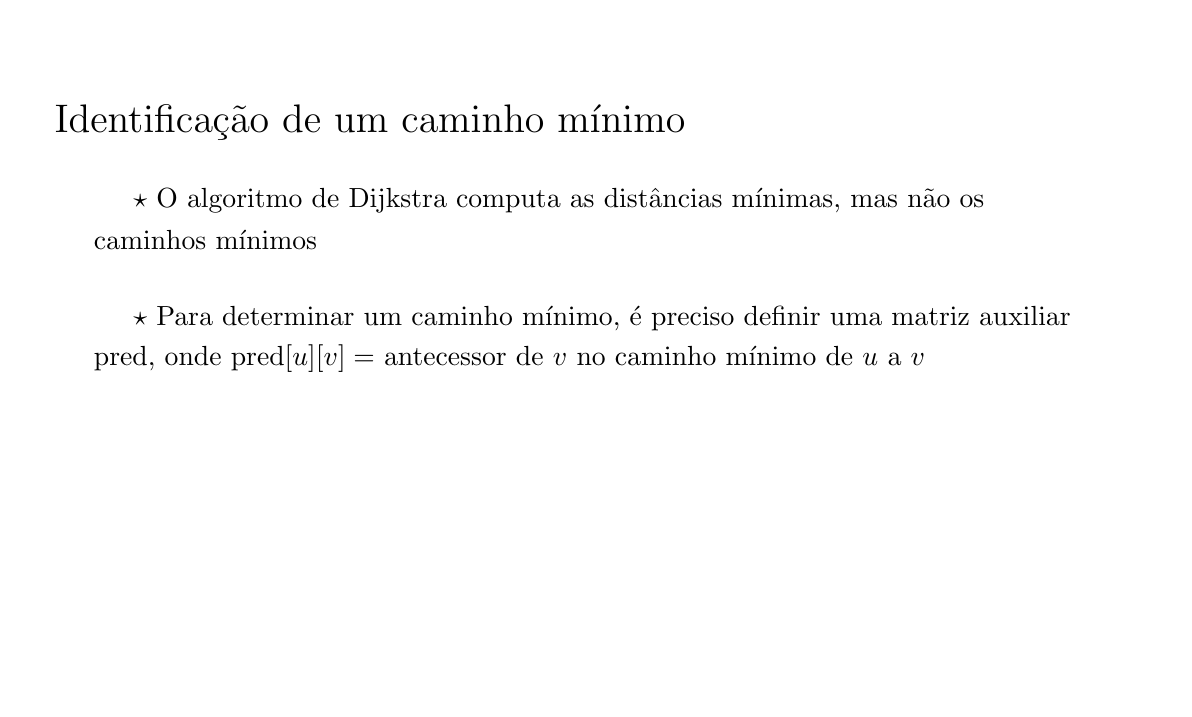
\begin{tikzpicture}
\node[draw,opacity=0] at (0, 0) {x};
\node[draw,opacity=0] at (14, 8) {x};

	\node[anchor=west] (title) at (0.0, 7.0) { \Large \bbbold{Identificação de um caminho mínimo} };


	\node[anchor=west] (a1) at (1.0, 6.0) { $\star$ \bbtext{O algoritmo de Dijkstra computa as distâncias mínimas, mas não os} };

	\node[anchor=west] (a2) at (0.5, 5.5) { \bbtext{caminhos mínimos} };


	\node[anchor=west] (b1) at (1.0, 4.5) { $\star$ \bbtext{Para determinar um caminho mínimo, é preciso definir uma matriz auxiliar} };

	\node[anchor=west] (b2) at (0.5, 4.0) { \bbtext{$\mathrm{pred}$, onde $\mathrm{pred}[u][v] = $ antecessor de $v$ no caminho mínimo de $u$ a $v$} };

\end{tikzpicture}
\end{frame}
\begin{frame}[plain,t]
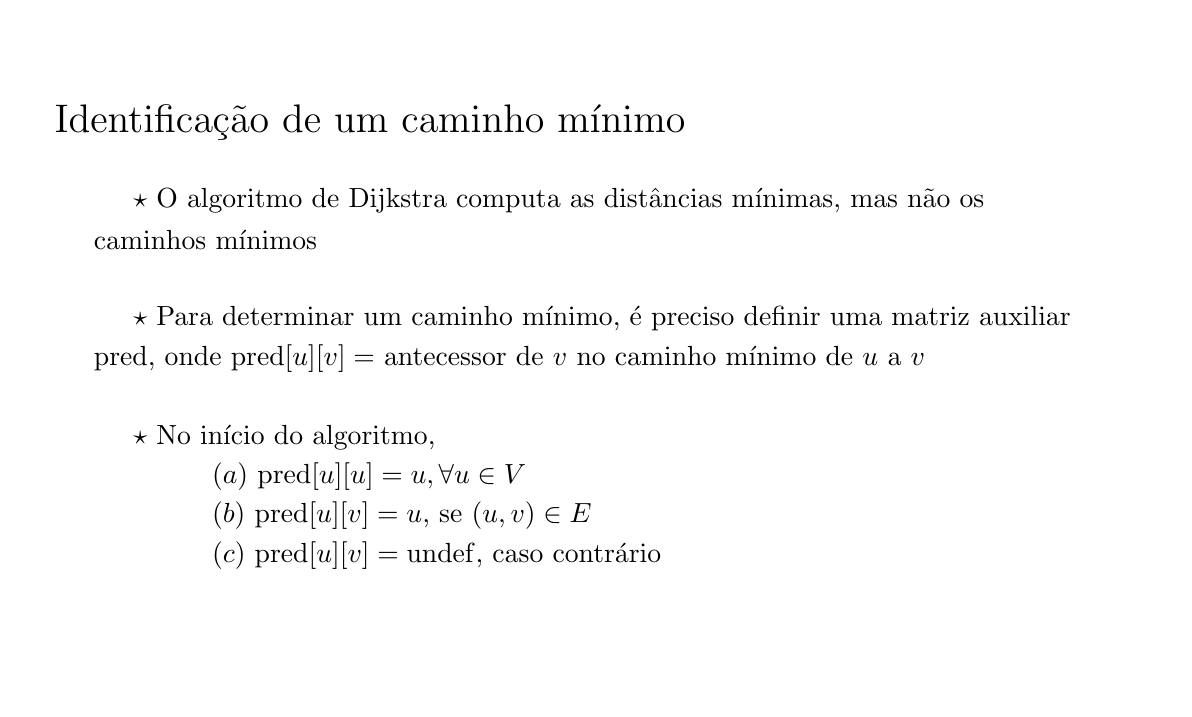
\begin{tikzpicture}
\node[draw,opacity=0] at (0, 0) {x};
\node[draw,opacity=0] at (14, 8) {x};

	\node[anchor=west] (title) at (0.0, 7.0) { \Large \bbbold{Identificação de um caminho mínimo} };


	\node[anchor=west] (a1) at (1.0, 6.0) { $\star$ \bbtext{O algoritmo de Dijkstra computa as distâncias mínimas, mas não os} };

	\node[anchor=west] (a2) at (0.5, 5.5) { \bbtext{caminhos mínimos} };


	\node[anchor=west] (b1) at (1.0, 4.5) { $\star$ \bbtext{Para determinar um caminho mínimo, é preciso definir uma matriz auxiliar} };

	\node[anchor=west] (b2) at (0.5, 4.0) { \bbtext{$\mathrm{pred}$, onde $\mathrm{pred}[u][v] = $ antecessor de $v$ no caminho mínimo de $u$ a $v$} };


	\node[anchor=west] (c1) at (1.0, 3.0) { $\star$ \bbtext{No início do algoritmo,} };

	\node[anchor=west] (c2) at (2.0, 2.5) { \bbtext{$(a)$ $\mathrm{pred}[u][u] = u, \forall u\in V$} };

	\node[anchor=west] (c3) at (2.0, 2.0) { \bbtext{$(b)$ $\mathrm{pred}[u][v] = u$, se $(u, v)\in E$} };

	\node[anchor=west] (c4) at (2.0, 1.5) { \bbtext{$(c)$ $\mathrm{pred}[u][v] = \mathrm{undef}$, caso contrário} };


\end{tikzpicture}
\end{frame}
\begin{frame}[plain,t]
\begin{tikzpicture}
\node[draw,opacity=0] at (0, 0) {x};
\node[draw,opacity=0] at (14, 8) {x};

	\node[anchor=west] (title) at (0.0, 6.0) { \Large \bbbold{Identificação de um caminho mínimo} };

\end{tikzpicture}
\end{frame}
\begin{frame}[plain,t]
\begin{tikzpicture}
\node[draw,opacity=0] at (0, 0) {x};
\node[draw,opacity=0] at (14, 8) {x};

	\node[anchor=west] (title) at (0.0, 6.0) { \Large \bbbold{Identificação de um caminho mínimo} };


	\node[anchor=west] (a) at (1.0, 5.0) { $\star$ \bbtext{Se $k$ atualizar $d[u][v]$, faça $\mathrm{pred}[u][v] = \mathrm{pred}[k][v]$} };


\end{tikzpicture}
\end{frame}
\begin{frame}[plain,t]
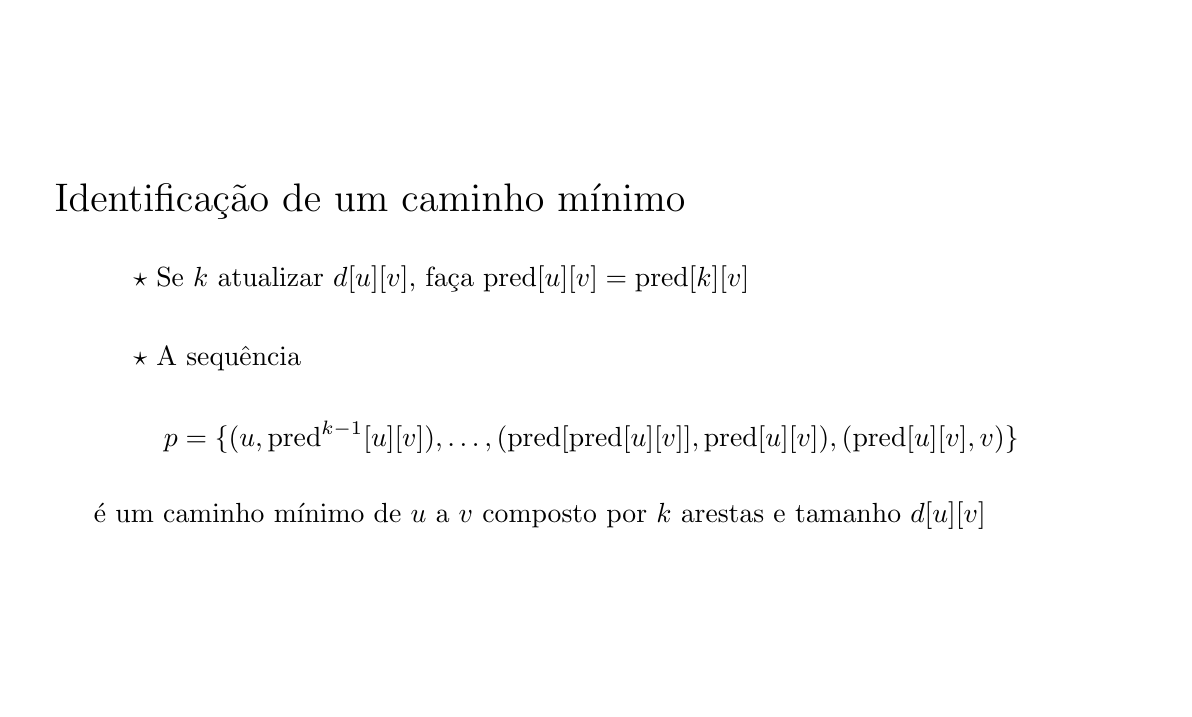
\begin{tikzpicture}
\node[draw,opacity=0] at (0, 0) {x};
\node[draw,opacity=0] at (14, 8) {x};

	\node[anchor=west] (title) at (0.0, 6.0) { \Large \bbbold{Identificação de um caminho mínimo} };


	\node[anchor=west] (a) at (1.0, 5.0) { $\star$ \bbtext{Se $k$ atualizar $d[u][v]$, faça $\mathrm{pred}[u][v] = \mathrm{pred}[k][v]$} };



	\node[anchor=west] (b1) at (1.0, 4.0) { $\star$ \bbtext{A sequência } };

	\node[] (b2) at (7.0, 3.0) { \bbtext{$ p = \{ (u, \mathrm{pred}^{k - 1}[u][v]), \ldots, (\mathrm{pred}[\mathrm{pred}[u][v]], \mathrm{pred}[u][v]), (\mathrm{pred}[u][v], v)\}$ } };

	\node[anchor=west] (b3) at (0.5, 2.0) { \bbtext{é um caminho mínimo de $u$ a $v$ composto por $k$ arestas e tamanho $d[u][v]$} };

\end{tikzpicture}
\end{frame}
\begin{frame}[plain,t]
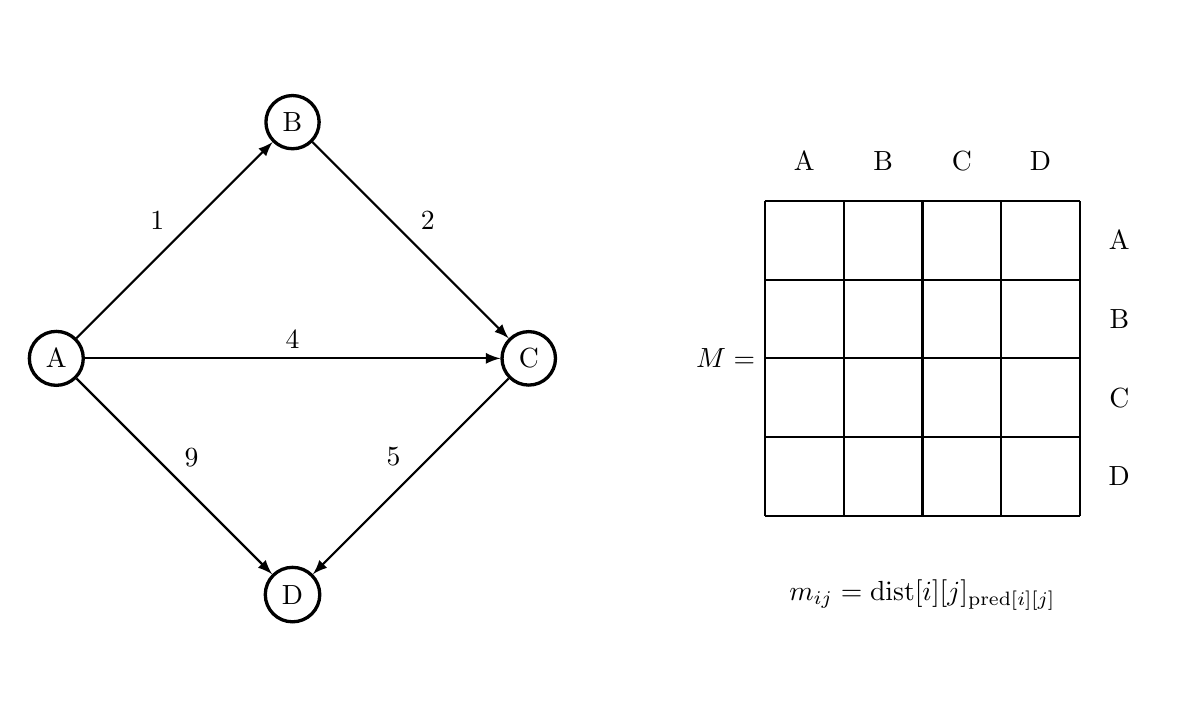
\begin{tikzpicture}
\node[draw,opacity=0] at (0, 0) {x};
\node[draw,opacity=0] at (14, 8) {x};

	\node[circle,draw,very thick] (a) at (0.0, 4.0) { \bbtext{A} };

	\node[circle,draw,very thick] (b) at (3.0, 7.0) { \bbtext{B} };

	\node[circle,draw,very thick] (c) at (6.0, 4.0) { \bbtext{C} };

	\node[circle,draw,very thick] (d) at (3.0, 1.0) { \bbtext{D} };

	\draw[-latex,thick](a) to node[above left] { \bbinfo{1} } (b);

	\draw[-latex,thick](a) to node[above] { \bbinfo{4} } (c);

	\draw[-latex,thick](a) to node[above right] { \bbinfo{9} } (d);

	\draw[-latex,thick](b) to node[above right] { \bbinfo{2} } (c);

	\draw[-latex,thick](c) to node[above left] { \bbinfo{5} } (d);

	\draw[thick] (9.0, 2.0) grid  (13.0, 6.0);

	\node[] (matrix) at (8.5, 4.0) { $M = $ };

	\node[] (legend) at (11.0, 1.0) { $m_{ij} = \mathrm{dist}[i][j]_{\mathrm{pred}[i][j]}$ };

	\node[] (r1) at (13.5, 5.5) { \bbtext{A} };

	\node[] (r2) at (13.5, 4.5) { \bbtext{B} };

	\node[] (r3) at (13.5, 3.5) { \bbtext{C} };

	\node[] (r4) at (13.5, 2.5) { \bbtext{D} };

	\node[] (c1) at (9.5, 6.5) { \bbtext{A} };

	\node[] (c2) at (10.5, 6.5) { \bbtext{B} };

	\node[] (c3) at (11.5, 6.5) { \bbtext{C} };

	\node[] (c4) at (12.5, 6.5) { \bbtext{D} };

\end{tikzpicture}
\end{frame}
\begin{frame}[plain,t]
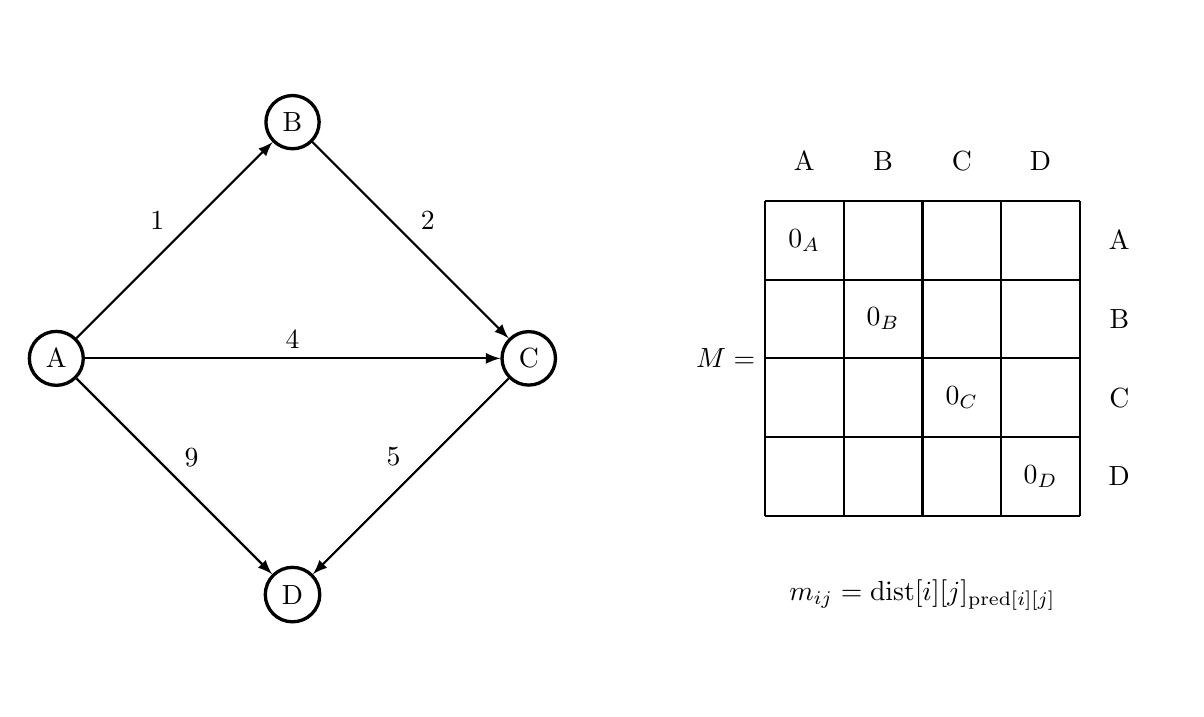
\begin{tikzpicture}
\node[draw,opacity=0] at (0, 0) {x};
\node[draw,opacity=0] at (14, 8) {x};

	\node[circle,draw,very thick] (a) at (0.0, 4.0) { \bbtext{A} };

	\node[circle,draw,very thick] (b) at (3.0, 7.0) { \bbtext{B} };

	\node[circle,draw,very thick] (c) at (6.0, 4.0) { \bbtext{C} };

	\node[circle,draw,very thick] (d) at (3.0, 1.0) { \bbtext{D} };

	\draw[-latex,thick](a) to node[above left] { \bbinfo{1} } (b);

	\draw[-latex,thick](a) to node[above] { \bbinfo{4} } (c);

	\draw[-latex,thick](a) to node[above right] { \bbinfo{9} } (d);

	\draw[-latex,thick](b) to node[above right] { \bbinfo{2} } (c);

	\draw[-latex,thick](c) to node[above left] { \bbinfo{5} } (d);

	\draw[thick] (9.0, 2.0) grid  (13.0, 6.0);

	\node[] (matrix) at (8.5, 4.0) { $M = $ };

	\node[] (legend) at (11.0, 1.0) { $m_{ij} = \mathrm{dist}[i][j]_{\mathrm{pred}[i][j]}$ };

	\node[] (r1) at (13.5, 5.5) { \bbtext{A} };

	\node[] (r2) at (13.5, 4.5) { \bbtext{B} };

	\node[] (r3) at (13.5, 3.5) { \bbtext{C} };

	\node[] (r4) at (13.5, 2.5) { \bbtext{D} };

	\node[] (c1) at (9.5, 6.5) { \bbtext{A} };

	\node[] (c2) at (10.5, 6.5) { \bbtext{B} };

	\node[] (c3) at (11.5, 6.5) { \bbtext{C} };

	\node[] (c4) at (12.5, 6.5) { \bbtext{D} };


	\node[] (a11) at (9.5, 5.5) { $\bbupdate{0}_{\bbtext{A}}$ };

	\node[] (a22) at (10.5, 4.5) { $\bbupdate{0}_{\bbtext{B}}$ };

	\node[] (a33) at (11.5, 3.5) { $\bbupdate{0}_{\bbtext{C}}$ };

	\node[] (a44) at (12.5, 2.5) { $\bbupdate{0}_{\bbtext{D}}$ };

\end{tikzpicture}
\end{frame}
\begin{frame}[plain,t]
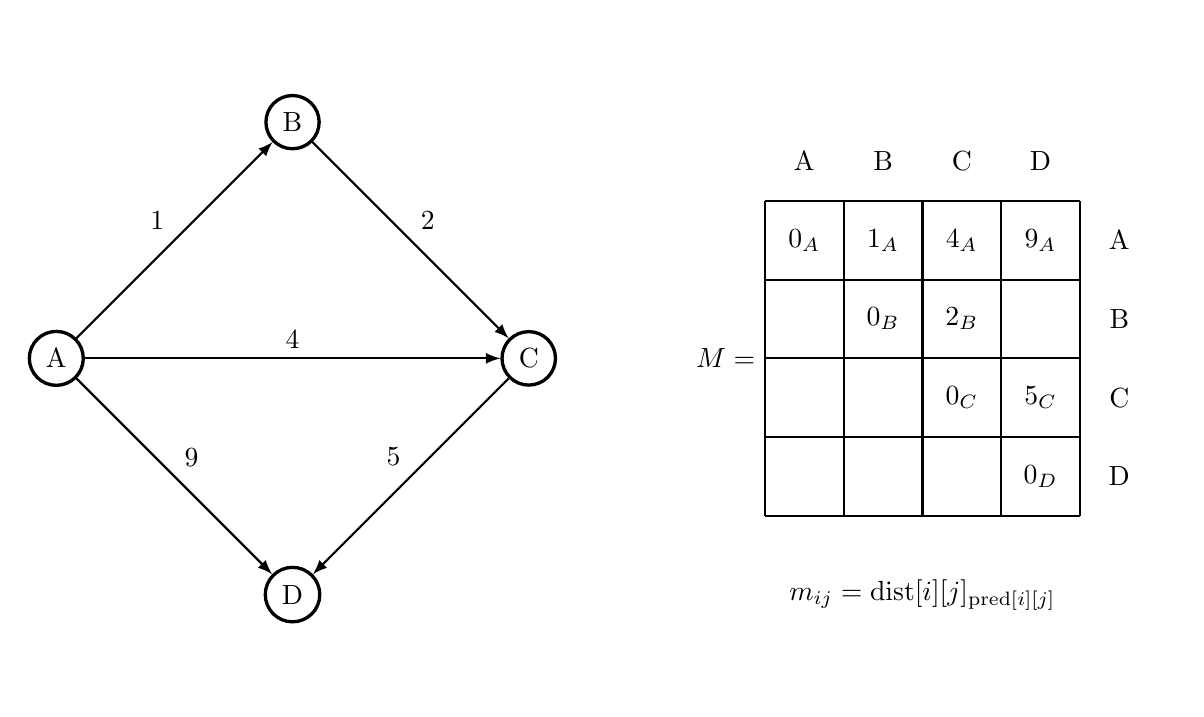
\begin{tikzpicture}
\node[draw,opacity=0] at (0, 0) {x};
\node[draw,opacity=0] at (14, 8) {x};

	\node[circle,draw,very thick] (a) at (0.0, 4.0) { \bbtext{A} };

	\node[circle,draw,very thick] (b) at (3.0, 7.0) { \bbtext{B} };

	\node[circle,draw,very thick] (c) at (6.0, 4.0) { \bbtext{C} };

	\node[circle,draw,very thick] (d) at (3.0, 1.0) { \bbtext{D} };

	\draw[-latex,thick](a) to node[above left] { \bbinfo{1} } (b);

	\draw[-latex,thick](a) to node[above] { \bbinfo{4} } (c);

	\draw[-latex,thick](a) to node[above right] { \bbinfo{9} } (d);

	\draw[-latex,thick](b) to node[above right] { \bbinfo{2} } (c);

	\draw[-latex,thick](c) to node[above left] { \bbinfo{5} } (d);

	\draw[thick] (9.0, 2.0) grid  (13.0, 6.0);

	\node[] (matrix) at (8.5, 4.0) { $M = $ };

	\node[] (legend) at (11.0, 1.0) { $m_{ij} = \mathrm{dist}[i][j]_{\mathrm{pred}[i][j]}$ };

	\node[] (r1) at (13.5, 5.5) { \bbtext{A} };

	\node[] (r2) at (13.5, 4.5) { \bbtext{B} };

	\node[] (r3) at (13.5, 3.5) { \bbtext{C} };

	\node[] (r4) at (13.5, 2.5) { \bbtext{D} };

	\node[] (c1) at (9.5, 6.5) { \bbtext{A} };

	\node[] (c2) at (10.5, 6.5) { \bbtext{B} };

	\node[] (c3) at (11.5, 6.5) { \bbtext{C} };

	\node[] (c4) at (12.5, 6.5) { \bbtext{D} };


	\node[] (a11) at (9.5, 5.5) { $0_{\bbtext{A}}$ };

	\node[] (a22) at (10.5, 4.5) { $0_{\bbtext{B}}$ };

	\node[] (a33) at (11.5, 3.5) { $0_{\bbtext{C}}$ };

	\node[] (a44) at (12.5, 2.5) { $0_{\bbtext{D}}$ };



	\node[] (a12) at (10.5, 5.5) { $\bbupdate{1}_{\bbtext{A}}$ };

	\node[] (a13) at (11.5, 5.5) { $\bbupdate{4}_{\bbtext{A}}$ };

	\node[] (a14) at (12.5, 5.5) { $\bbupdate{9}_{\bbtext{A}}$ };

	\node[] (b23) at (11.5, 4.5) { $\bbupdate{2}_{\bbtext{B}}$ };

	\node[] (c34) at (12.5, 3.5) { $\bbupdate{5}_{\bbtext{C}}$ };

\end{tikzpicture}
\end{frame}
\begin{frame}[plain,t]
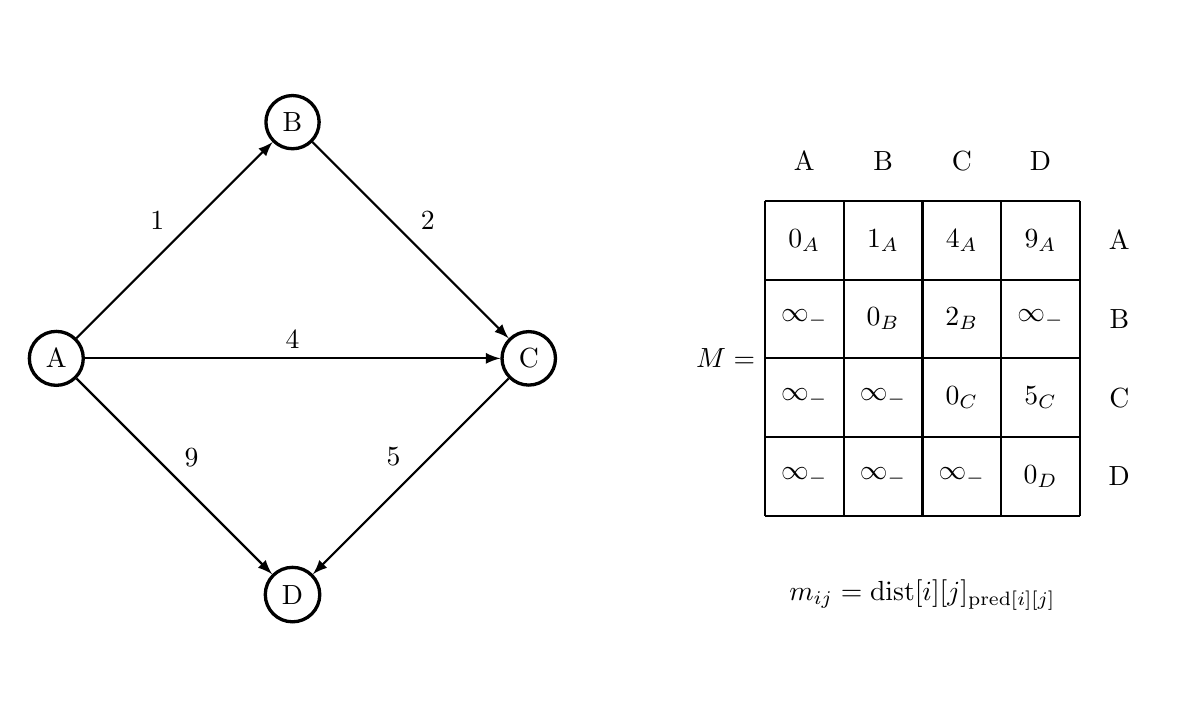
\begin{tikzpicture}
\node[draw,opacity=0] at (0, 0) {x};
\node[draw,opacity=0] at (14, 8) {x};

	\node[circle,draw,very thick] (a) at (0.0, 4.0) { \bbtext{A} };

	\node[circle,draw,very thick] (b) at (3.0, 7.0) { \bbtext{B} };

	\node[circle,draw,very thick] (c) at (6.0, 4.0) { \bbtext{C} };

	\node[circle,draw,very thick] (d) at (3.0, 1.0) { \bbtext{D} };

	\draw[-latex,thick](a) to node[above left] { \bbinfo{1} } (b);

	\draw[-latex,thick](a) to node[above] { \bbinfo{4} } (c);

	\draw[-latex,thick](a) to node[above right] { \bbinfo{9} } (d);

	\draw[-latex,thick](b) to node[above right] { \bbinfo{2} } (c);

	\draw[-latex,thick](c) to node[above left] { \bbinfo{5} } (d);

	\draw[thick] (9.0, 2.0) grid  (13.0, 6.0);

	\node[] (matrix) at (8.5, 4.0) { $M = $ };

	\node[] (legend) at (11.0, 1.0) { $m_{ij} = \mathrm{dist}[i][j]_{\mathrm{pred}[i][j]}$ };

	\node[] (r1) at (13.5, 5.5) { \bbtext{A} };

	\node[] (r2) at (13.5, 4.5) { \bbtext{B} };

	\node[] (r3) at (13.5, 3.5) { \bbtext{C} };

	\node[] (r4) at (13.5, 2.5) { \bbtext{D} };

	\node[] (c1) at (9.5, 6.5) { \bbtext{A} };

	\node[] (c2) at (10.5, 6.5) { \bbtext{B} };

	\node[] (c3) at (11.5, 6.5) { \bbtext{C} };

	\node[] (c4) at (12.5, 6.5) { \bbtext{D} };


	\node[] (a11) at (9.5, 5.5) { $0_{\bbtext{A}}$ };

	\node[] (a22) at (10.5, 4.5) { $0_{\bbtext{B}}$ };

	\node[] (a33) at (11.5, 3.5) { $0_{\bbtext{C}}$ };

	\node[] (a44) at (12.5, 2.5) { $0_{\bbtext{D}}$ };



	\node[] (a12) at (10.5, 5.5) { $1_{\bbtext{A}}$ };

	\node[] (a13) at (11.5, 5.5) { $4_{\bbtext{A}}$ };

	\node[] (a14) at (12.5, 5.5) { $9_{\bbtext{A}}$ };

	\node[] (b23) at (11.5, 4.5) { $2_{\bbtext{B}}$ };

	\node[] (c34) at (12.5, 3.5) { $5_{\bbtext{C}}$ };



	\node[] (b21) at (9.5, 4.5) { $\bbupdate{\infty}_{\bbtext{-}}$ };

	\node[] (b24) at (12.5, 4.5) { $\bbupdate{\infty}_{\bbtext{-}}$ };

	\node[] (c31) at (9.5, 3.5) { $\bbupdate{\infty}_{\bbtext{-}}$ };

	\node[] (c32) at (10.5, 3.5) { $\bbupdate{\infty}_{\bbtext{-}}$ };

	\node[] (d41) at (9.5, 2.5) { $\bbupdate{\infty}_{\bbtext{-}}$ };

	\node[] (d42) at (10.5, 2.5) { $\bbupdate{\infty}_{\bbtext{-}}$ };

	\node[] (d43) at (11.5, 2.5) { $\bbupdate{\infty}_{\bbtext{-}}$ };

\end{tikzpicture}
\end{frame}
\begin{frame}[plain,t]
\begin{tikzpicture}
\node[draw,opacity=0] at (0, 0) {x};
\node[draw,opacity=0] at (14, 8) {x};

	\node[circle,draw,very thick,fill=BBGreen] (a) at (0.0, 4.0) { \bbtext{A} };

	\node[circle,draw,very thick] (b) at (3.0, 7.0) { \bbtext{B} };

	\node[circle,draw,very thick] (c) at (6.0, 4.0) { \bbtext{C} };

	\node[circle,draw,very thick] (d) at (3.0, 1.0) { \bbtext{D} };

	\draw[-latex,thick](a) to node[above left] { \bbinfo{1} } (b);

	\draw[-latex,thick](a) to node[above] { \bbinfo{4} } (c);

	\draw[-latex,thick](a) to node[above right] { \bbinfo{9} } (d);

	\draw[-latex,thick](b) to node[above right] { \bbinfo{2} } (c);

	\draw[-latex,thick](c) to node[above left] { \bbinfo{5} } (d);

	\draw[thick] (9.0, 2.0) grid  (13.0, 6.0);

	\node[] (matrix) at (8.5, 4.0) { $M = $ };

	\node[] (legend) at (11.0, 1.0) { $m_{ij} = \mathrm{dist}[i][j]_{\mathrm{pred}[i][j]}$ };

	\node[] (r1) at (13.5, 5.5) { \bbtext{A} };

	\node[] (r2) at (13.5, 4.5) { \bbtext{B} };

	\node[] (r3) at (13.5, 3.5) { \bbtext{C} };

	\node[] (r4) at (13.5, 2.5) { \bbtext{D} };

	\node[] (c1) at (9.5, 6.5) { \bbtext{A} };

	\node[] (c2) at (10.5, 6.5) { \bbtext{B} };

	\node[] (c3) at (11.5, 6.5) { \bbtext{C} };

	\node[] (c4) at (12.5, 6.5) { \bbtext{D} };


	\node[] (a11) at (9.5, 5.5) { $0_{\bbtext{A}}$ };

	\node[] (a22) at (10.5, 4.5) { $0_{\bbtext{B}}$ };

	\node[] (a33) at (11.5, 3.5) { $0_{\bbtext{C}}$ };

	\node[] (a44) at (12.5, 2.5) { $0_{\bbtext{D}}$ };



	\node[] (a12) at (10.5, 5.5) { $1_{\bbtext{A}}$ };

	\node[] (a13) at (11.5, 5.5) { $4_{\bbtext{A}}$ };

	\node[] (a14) at (12.5, 5.5) { $9_{\bbtext{A}}$ };

	\node[] (b23) at (11.5, 4.5) { $2_{\bbtext{B}}$ };

	\node[] (c34) at (12.5, 3.5) { $5_{\bbtext{C}}$ };



	\node[] (b21) at (9.5, 4.5) { $\bbupdate{\infty}_{\bbtext{-}}$ };

	\node[] (b24) at (12.5, 4.5) { $\bbupdate{\infty}_{\bbtext{-}}$ };

	\node[] (c31) at (9.5, 3.5) { $\bbupdate{\infty}_{\bbtext{-}}$ };

	\node[] (c32) at (10.5, 3.5) { $\bbupdate{\infty}_{\bbtext{-}}$ };

	\node[] (d41) at (9.5, 2.5) { $\bbupdate{\infty}_{\bbtext{-}}$ };

	\node[] (d42) at (10.5, 2.5) { $\bbupdate{\infty}_{\bbtext{-}}$ };

	\node[] (d43) at (11.5, 2.5) { $\bbupdate{\infty}_{\bbtext{-}}$ };



\end{tikzpicture}
\end{frame}
\begin{frame}[plain,t]
\begin{tikzpicture}
\node[draw,opacity=0] at (0, 0) {x};
\node[draw,opacity=0] at (14, 8) {x};

	\node[circle,draw,very thick,fill=BBCyan] (a) at (0.0, 4.0) { \bbtext{A} };

	\node[circle,draw,very thick,fill=BBGreen] (b) at (3.0, 7.0) { \bbtext{B} };

	\node[circle,draw,very thick] (c) at (6.0, 4.0) { \bbtext{C} };

	\node[circle,draw,very thick] (d) at (3.0, 1.0) { \bbtext{D} };

	\draw[-latex,thick](a) to node[above left] { \bbinfo{1} } (b);

	\draw[-latex,thick](a) to node[above] { \bbinfo{4} } (c);

	\draw[-latex,thick](a) to node[above right] { \bbinfo{9} } (d);

	\draw[-latex,thick](b) to node[above right] { \bbinfo{2} } (c);

	\draw[-latex,thick](c) to node[above left] { \bbinfo{5} } (d);

	\draw[thick] (9.0, 2.0) grid  (13.0, 6.0);

	\node[] (matrix) at (8.5, 4.0) { $M = $ };

	\node[] (legend) at (11.0, 1.0) { $m_{ij} = \mathrm{dist}[i][j]_{\mathrm{pred}[i][j]}$ };

	\node[] (r1) at (13.5, 5.5) { \bbtext{A} };

	\node[] (r2) at (13.5, 4.5) { \bbtext{B} };

	\node[] (r3) at (13.5, 3.5) { \bbtext{C} };

	\node[] (r4) at (13.5, 2.5) { \bbtext{D} };

	\node[] (c1) at (9.5, 6.5) { \bbtext{A} };

	\node[] (c2) at (10.5, 6.5) { \bbtext{B} };

	\node[] (c3) at (11.5, 6.5) { \bbtext{C} };

	\node[] (c4) at (12.5, 6.5) { \bbtext{D} };


	\node[] (a11) at (9.5, 5.5) { $0_{\bbtext{A}}$ };

	\node[] (a22) at (10.5, 4.5) { $0_{\bbtext{B}}$ };

	\node[] (a33) at (11.5, 3.5) { $0_{\bbtext{C}}$ };

	\node[] (a44) at (12.5, 2.5) { $0_{\bbtext{D}}$ };



	\node[] (a12) at (10.5, 5.5) { $1_{\bbtext{A}}$ };

	\node[] (a13) at (11.5, 5.5) { $\bbupdate{3}_{\bbtext{\bbupdate{B}}}$ };

	\node[] (a14) at (12.5, 5.5) { $9_{\bbtext{A}}$ };

	\node[] (b23) at (11.5, 4.5) { $2_{\bbtext{B}}$ };

	\node[] (c34) at (12.5, 3.5) { $5_{\bbtext{C}}$ };



	\node[] (b21) at (9.5, 4.5) { $\bbupdate{\infty}_{\bbtext{-}}$ };

	\node[] (b24) at (12.5, 4.5) { $\bbupdate{\infty}_{\bbtext{-}}$ };

	\node[] (c31) at (9.5, 3.5) { $\bbupdate{\infty}_{\bbtext{-}}$ };

	\node[] (c32) at (10.5, 3.5) { $\bbupdate{\infty}_{\bbtext{-}}$ };

	\node[] (d41) at (9.5, 2.5) { $\bbupdate{\infty}_{\bbtext{-}}$ };

	\node[] (d42) at (10.5, 2.5) { $\bbupdate{\infty}_{\bbtext{-}}$ };

	\node[] (d43) at (11.5, 2.5) { $\bbupdate{\infty}_{\bbtext{-}}$ };






\end{tikzpicture}
\end{frame}
\begin{frame}[plain,t]
\begin{tikzpicture}
\node[draw,opacity=0] at (0, 0) {x};
\node[draw,opacity=0] at (14, 8) {x};

	\node[circle,draw,very thick,fill=BBCyan] (a) at (0.0, 4.0) { \bbtext{A} };

	\node[circle,draw,very thick,fill=BBCyan] (b) at (3.0, 7.0) { \bbtext{B} };

	\node[circle,draw,very thick,fill=BBGreen] (c) at (6.0, 4.0) { \bbtext{C} };

	\node[circle,draw,very thick] (d) at (3.0, 1.0) { \bbtext{D} };

	\draw[-latex,thick](a) to node[above left] { \bbinfo{1} } (b);

	\draw[-latex,thick](a) to node[above] { \bbinfo{4} } (c);

	\draw[-latex,thick](a) to node[above right] { \bbinfo{9} } (d);

	\draw[-latex,thick](b) to node[above right] { \bbinfo{2} } (c);

	\draw[-latex,thick](c) to node[above left] { \bbinfo{5} } (d);

	\draw[thick] (9.0, 2.0) grid  (13.0, 6.0);

	\node[] (matrix) at (8.5, 4.0) { $M = $ };

	\node[] (legend) at (11.0, 1.0) { $m_{ij} = \mathrm{dist}[i][j]_{\mathrm{pred}[i][j]}$ };

	\node[] (r1) at (13.5, 5.5) { \bbtext{A} };

	\node[] (r2) at (13.5, 4.5) { \bbtext{B} };

	\node[] (r3) at (13.5, 3.5) { \bbtext{C} };

	\node[] (r4) at (13.5, 2.5) { \bbtext{D} };

	\node[] (c1) at (9.5, 6.5) { \bbtext{A} };

	\node[] (c2) at (10.5, 6.5) { \bbtext{B} };

	\node[] (c3) at (11.5, 6.5) { \bbtext{C} };

	\node[] (c4) at (12.5, 6.5) { \bbtext{D} };


	\node[] (a11) at (9.5, 5.5) { $0_{\bbtext{A}}$ };

	\node[] (a22) at (10.5, 4.5) { $0_{\bbtext{B}}$ };

	\node[] (a33) at (11.5, 3.5) { $0_{\bbtext{C}}$ };

	\node[] (a44) at (12.5, 2.5) { $0_{\bbtext{D}}$ };



	\node[] (a12) at (10.5, 5.5) { $1_{\bbtext{A}}$ };

	\node[] (a13) at (11.5, 5.5) { ${3}_{\bbtext{{B}}}$ };

	\node[] (a14) at (12.5, 5.5) { $\bbupdate{8}_{\bbtext{\bbupdate{C}}}$ };

	\node[] (b23) at (11.5, 4.5) { $2_{\bbtext{B}}$ };

	\node[] (c34) at (12.5, 3.5) { $5_{\bbtext{C}}$ };



	\node[] (b21) at (9.5, 4.5) { $\bbupdate{\infty}_{\bbtext{-}}$ };

	\node[] (b24) at (12.5, 4.5) { $\bbupdate{7}_{\bbtext{\bbupdate{C}}}$ };

	\node[] (c31) at (9.5, 3.5) { $\bbupdate{\infty}_{\bbtext{-}}$ };

	\node[] (c32) at (10.5, 3.5) { $\bbupdate{\infty}_{\bbtext{-}}$ };

	\node[] (d41) at (9.5, 2.5) { $\bbupdate{\infty}_{\bbtext{-}}$ };

	\node[] (d42) at (10.5, 2.5) { $\bbupdate{\infty}_{\bbtext{-}}$ };

	\node[] (d43) at (11.5, 2.5) { $\bbupdate{\infty}_{\bbtext{-}}$ };









\end{tikzpicture}
\end{frame}
\begin{frame}[plain,t]
\begin{tikzpicture}
\node[draw,opacity=0] at (0, 0) {x};
\node[draw,opacity=0] at (14, 8) {x};

	\node[circle,draw,very thick,fill=BBCyan] (a) at (0.0, 4.0) { \bbtext{A} };

	\node[circle,draw,very thick,fill=BBCyan] (b) at (3.0, 7.0) { \bbtext{B} };

	\node[circle,draw,very thick,fill=BBCyan] (c) at (6.0, 4.0) { \bbtext{C} };

	\node[circle,draw,very thick,fill=BBGreen] (d) at (3.0, 1.0) { \bbtext{D} };

	\draw[-latex,thick](a) to node[above left] { \bbinfo{1} } (b);

	\draw[-latex,thick](a) to node[above] { \bbinfo{4} } (c);

	\draw[-latex,thick](a) to node[above right] { \bbinfo{9} } (d);

	\draw[-latex,thick](b) to node[above right] { \bbinfo{2} } (c);

	\draw[-latex,thick](c) to node[above left] { \bbinfo{5} } (d);

	\draw[thick] (9.0, 2.0) grid  (13.0, 6.0);

	\node[] (matrix) at (8.5, 4.0) { $M = $ };

	\node[] (legend) at (11.0, 1.0) { $m_{ij} = \mathrm{dist}[i][j]_{\mathrm{pred}[i][j]}$ };

	\node[] (r1) at (13.5, 5.5) { \bbtext{A} };

	\node[] (r2) at (13.5, 4.5) { \bbtext{B} };

	\node[] (r3) at (13.5, 3.5) { \bbtext{C} };

	\node[] (r4) at (13.5, 2.5) { \bbtext{D} };

	\node[] (c1) at (9.5, 6.5) { \bbtext{A} };

	\node[] (c2) at (10.5, 6.5) { \bbtext{B} };

	\node[] (c3) at (11.5, 6.5) { \bbtext{C} };

	\node[] (c4) at (12.5, 6.5) { \bbtext{D} };


	\node[] (a11) at (9.5, 5.5) { $0_{\bbtext{A}}$ };

	\node[] (a22) at (10.5, 4.5) { $0_{\bbtext{B}}$ };

	\node[] (a33) at (11.5, 3.5) { $0_{\bbtext{C}}$ };

	\node[] (a44) at (12.5, 2.5) { $0_{\bbtext{D}}$ };



	\node[] (a12) at (10.5, 5.5) { $1_{\bbtext{A}}$ };

	\node[] (a13) at (11.5, 5.5) { ${3}_{\bbtext{{B}}}$ };

	\node[] (a14) at (12.5, 5.5) { ${8}_{\bbtext{{C}}}$ };

	\node[] (b23) at (11.5, 4.5) { $2_{\bbtext{B}}$ };

	\node[] (c34) at (12.5, 3.5) { $5_{\bbtext{C}}$ };



	\node[] (b21) at (9.5, 4.5) { $\bbupdate{\infty}_{\bbtext{-}}$ };

	\node[] (b24) at (12.5, 4.5) { ${7}_{\bbtext{{C}}}$ };

	\node[] (c31) at (9.5, 3.5) { $\bbupdate{\infty}_{\bbtext{-}}$ };

	\node[] (c32) at (10.5, 3.5) { $\bbupdate{\infty}_{\bbtext{-}}$ };

	\node[] (d41) at (9.5, 2.5) { $\bbupdate{\infty}_{\bbtext{-}}$ };

	\node[] (d42) at (10.5, 2.5) { $\bbupdate{\infty}_{\bbtext{-}}$ };

	\node[] (d43) at (11.5, 2.5) { $\bbupdate{\infty}_{\bbtext{-}}$ };












\end{tikzpicture}
\end{frame}
\begin{frame}[plain,t]
\begin{tikzpicture}
\node[draw,opacity=0] at (0, 0) {x};
\node[draw,opacity=0] at (14, 8) {x};

	\node[circle,draw,very thick,fill=BBCyan] (a) at (0.0, 4.0) { \bbtext{A} };

	\node[circle,draw,very thick,fill=BBCyan] (b) at (3.0, 7.0) { \bbtext{B} };

	\node[circle,draw,very thick,fill=BBCyan] (c) at (6.0, 4.0) { \bbtext{C} };

	\node[circle,draw,very thick,fill=BBGreen] (d) at (3.0, 1.0) { \bbtext{D} };

	\draw[-latex,thick](a) to node[above left] { \bbinfo{1} } (b);

	\draw[-latex,thick](a) to node[above] { \bbinfo{4} } (c);

	\draw[-latex,thick](a) to node[above right] { \bbinfo{9} } (d);

	\draw[-latex,thick](b) to node[above right] { \bbinfo{2} } (c);

	\draw[-latex,thick](c) to node[above left] { \bbinfo{5} } (d);

	\draw[thick] (9.0, 2.0) grid  (13.0, 6.0);

	\node[] (matrix) at (8.5, 4.0) { $M = $ };

	\node[] (legend) at (11.0, 1.0) { $m_{ij} = \mathrm{dist}[i][j]_{\mathrm{pred}[i][j]}$ };

	\node[] (r1) at (13.5, 5.5) { \bbtext{A} };

	\node[] (r2) at (13.5, 4.5) { \bbtext{B} };

	\node[] (r3) at (13.5, 3.5) { \bbtext{C} };

	\node[] (r4) at (13.5, 2.5) { \bbtext{D} };

	\node[] (c1) at (9.5, 6.5) { \bbtext{A} };

	\node[] (c2) at (10.5, 6.5) { \bbtext{B} };

	\node[] (c3) at (11.5, 6.5) { \bbtext{C} };

	\node[] (c4) at (12.5, 6.5) { \bbtext{D} };


	\node[] (a11) at (9.5, 5.5) { $0_{\bbtext{A}}$ };

	\node[] (a22) at (10.5, 4.5) { $0_{\bbtext{B}}$ };

	\node[] (a33) at (11.5, 3.5) { $0_{\bbtext{C}}$ };

	\node[] (a44) at (12.5, 2.5) { $0_{\bbtext{D}}$ };



	\node[] (a12) at (10.5, 5.5) { $1_{\bbtext{A}}$ };

	\node[] (a13) at (11.5, 5.5) { ${3}_{\bbtext{{B}}}$ };

	\node[] (a14) at (12.5, 5.5) { ${8}_{\bbtext{{C}}}$ };

	\node[] (b23) at (11.5, 4.5) { $2_{\bbtext{B}}$ };

	\node[] (c34) at (12.5, 3.5) { $5_{\bbtext{C}}$ };



	\node[] (b21) at (9.5, 4.5) { $\bbupdate{\infty}_{\bbtext{-}}$ };

	\node[] (b24) at (12.5, 4.5) { ${7}_{\bbtext{{C}}}$ };

	\node[] (c31) at (9.5, 3.5) { $\bbupdate{\infty}_{\bbtext{-}}$ };

	\node[] (c32) at (10.5, 3.5) { $\bbupdate{\infty}_{\bbtext{-}}$ };

	\node[] (d41) at (9.5, 2.5) { $\bbupdate{\infty}_{\bbtext{-}}$ };

	\node[] (d42) at (10.5, 2.5) { $\bbupdate{\infty}_{\bbtext{-}}$ };

	\node[] (d43) at (11.5, 2.5) { $\bbupdate{\infty}_{\bbtext{-}}$ };













	\draw[color=BBViolet,latex-,dashed](d) to [bend right] node[below right, pos=0.3] { \tiny $(\mathrm{prev}[\mbox{\bbtext{A}}][\mbox{\bbtext{D}}], \mbox{\bbtext{D}})$ } (c);

\end{tikzpicture}
\end{frame}
\begin{frame}[plain,t]
\begin{tikzpicture}
\node[draw,opacity=0] at (0, 0) {x};
\node[draw,opacity=0] at (14, 8) {x};

	\node[circle,draw,very thick,fill=BBCyan] (a) at (0.0, 4.0) { \bbtext{A} };

	\node[circle,draw,very thick,fill=BBCyan] (b) at (3.0, 7.0) { \bbtext{B} };

	\node[circle,draw,very thick,fill=BBCyan] (c) at (6.0, 4.0) { \bbtext{C} };

	\node[circle,draw,very thick,fill=BBGreen] (d) at (3.0, 1.0) { \bbtext{D} };

	\draw[-latex,thick](a) to node[above left] { \bbinfo{1} } (b);

	\draw[-latex,thick](a) to node[above] { \bbinfo{4} } (c);

	\draw[-latex,thick](a) to node[above right] { \bbinfo{9} } (d);

	\draw[-latex,thick](b) to node[above right] { \bbinfo{2} } (c);

	\draw[-latex,thick](c) to node[above left] { \bbinfo{5} } (d);

	\draw[thick] (9.0, 2.0) grid  (13.0, 6.0);

	\node[] (matrix) at (8.5, 4.0) { $M = $ };

	\node[] (legend) at (11.0, 1.0) { $m_{ij} = \mathrm{dist}[i][j]_{\mathrm{pred}[i][j]}$ };

	\node[] (r1) at (13.5, 5.5) { \bbtext{A} };

	\node[] (r2) at (13.5, 4.5) { \bbtext{B} };

	\node[] (r3) at (13.5, 3.5) { \bbtext{C} };

	\node[] (r4) at (13.5, 2.5) { \bbtext{D} };

	\node[] (c1) at (9.5, 6.5) { \bbtext{A} };

	\node[] (c2) at (10.5, 6.5) { \bbtext{B} };

	\node[] (c3) at (11.5, 6.5) { \bbtext{C} };

	\node[] (c4) at (12.5, 6.5) { \bbtext{D} };


	\node[] (a11) at (9.5, 5.5) { $0_{\bbtext{A}}$ };

	\node[] (a22) at (10.5, 4.5) { $0_{\bbtext{B}}$ };

	\node[] (a33) at (11.5, 3.5) { $0_{\bbtext{C}}$ };

	\node[] (a44) at (12.5, 2.5) { $0_{\bbtext{D}}$ };



	\node[] (a12) at (10.5, 5.5) { $1_{\bbtext{A}}$ };

	\node[] (a13) at (11.5, 5.5) { ${3}_{\bbtext{{B}}}$ };

	\node[] (a14) at (12.5, 5.5) { ${8}_{\bbtext{{C}}}$ };

	\node[] (b23) at (11.5, 4.5) { $2_{\bbtext{B}}$ };

	\node[] (c34) at (12.5, 3.5) { $5_{\bbtext{C}}$ };



	\node[] (b21) at (9.5, 4.5) { $\bbupdate{\infty}_{\bbtext{-}}$ };

	\node[] (b24) at (12.5, 4.5) { ${7}_{\bbtext{{C}}}$ };

	\node[] (c31) at (9.5, 3.5) { $\bbupdate{\infty}_{\bbtext{-}}$ };

	\node[] (c32) at (10.5, 3.5) { $\bbupdate{\infty}_{\bbtext{-}}$ };

	\node[] (d41) at (9.5, 2.5) { $\bbupdate{\infty}_{\bbtext{-}}$ };

	\node[] (d42) at (10.5, 2.5) { $\bbupdate{\infty}_{\bbtext{-}}$ };

	\node[] (d43) at (11.5, 2.5) { $\bbupdate{\infty}_{\bbtext{-}}$ };













	\draw[color=BBViolet,latex-,dashed](d) to [bend right] node[below right, pos=0.3] { \tiny $(\mathrm{prev}[\mbox{\bbtext{A}}][\mbox{\bbtext{D}}], \mbox{\bbtext{D}})$ } (c);


	\draw[color=BBViolet,latex-,dashed](c) to [bend right] node[above right, pos=0.3] { \tiny $(\mathrm{prev}[\bbtext{A}][\mbox{\bbtext{C}}], \mbox{\bbtext{C}})$ } (b);

\end{tikzpicture}
\end{frame}
\begin{frame}[plain,t]
\begin{tikzpicture}
\node[draw,opacity=0] at (0, 0) {x};
\node[draw,opacity=0] at (14, 8) {x};

	\node[circle,draw,very thick,fill=BBCyan] (a) at (0.0, 4.0) { \bbtext{A} };

	\node[circle,draw,very thick,fill=BBCyan] (b) at (3.0, 7.0) { \bbtext{B} };

	\node[circle,draw,very thick,fill=BBCyan] (c) at (6.0, 4.0) { \bbtext{C} };

	\node[circle,draw,very thick,fill=BBGreen] (d) at (3.0, 1.0) { \bbtext{D} };

	\draw[-latex,thick](a) to node[above left] { \bbinfo{1} } (b);

	\draw[-latex,thick](a) to node[above] { \bbinfo{4} } (c);

	\draw[-latex,thick](a) to node[above right] { \bbinfo{9} } (d);

	\draw[-latex,thick](b) to node[above right] { \bbinfo{2} } (c);

	\draw[-latex,thick](c) to node[above left] { \bbinfo{5} } (d);

	\draw[thick] (9.0, 2.0) grid  (13.0, 6.0);

	\node[] (matrix) at (8.5, 4.0) { $M = $ };

	\node[] (legend) at (11.0, 1.0) { $m_{ij} = \mathrm{dist}[i][j]_{\mathrm{pred}[i][j]}$ };

	\node[] (r1) at (13.5, 5.5) { \bbtext{A} };

	\node[] (r2) at (13.5, 4.5) { \bbtext{B} };

	\node[] (r3) at (13.5, 3.5) { \bbtext{C} };

	\node[] (r4) at (13.5, 2.5) { \bbtext{D} };

	\node[] (c1) at (9.5, 6.5) { \bbtext{A} };

	\node[] (c2) at (10.5, 6.5) { \bbtext{B} };

	\node[] (c3) at (11.5, 6.5) { \bbtext{C} };

	\node[] (c4) at (12.5, 6.5) { \bbtext{D} };


	\node[] (a11) at (9.5, 5.5) { $0_{\bbtext{A}}$ };

	\node[] (a22) at (10.5, 4.5) { $0_{\bbtext{B}}$ };

	\node[] (a33) at (11.5, 3.5) { $0_{\bbtext{C}}$ };

	\node[] (a44) at (12.5, 2.5) { $0_{\bbtext{D}}$ };



	\node[] (a12) at (10.5, 5.5) { $1_{\bbtext{A}}$ };

	\node[] (a13) at (11.5, 5.5) { ${3}_{\bbtext{{B}}}$ };

	\node[] (a14) at (12.5, 5.5) { ${8}_{\bbtext{{C}}}$ };

	\node[] (b23) at (11.5, 4.5) { $2_{\bbtext{B}}$ };

	\node[] (c34) at (12.5, 3.5) { $5_{\bbtext{C}}$ };



	\node[] (b21) at (9.5, 4.5) { $\bbupdate{\infty}_{\bbtext{-}}$ };

	\node[] (b24) at (12.5, 4.5) { ${7}_{\bbtext{{C}}}$ };

	\node[] (c31) at (9.5, 3.5) { $\bbupdate{\infty}_{\bbtext{-}}$ };

	\node[] (c32) at (10.5, 3.5) { $\bbupdate{\infty}_{\bbtext{-}}$ };

	\node[] (d41) at (9.5, 2.5) { $\bbupdate{\infty}_{\bbtext{-}}$ };

	\node[] (d42) at (10.5, 2.5) { $\bbupdate{\infty}_{\bbtext{-}}$ };

	\node[] (d43) at (11.5, 2.5) { $\bbupdate{\infty}_{\bbtext{-}}$ };













	\draw[color=BBViolet,latex-,dashed](d) to [bend right] node[below right, pos=0.3] { \tiny $(\mathrm{prev}[\mbox{\bbtext{A}}][\mbox{\bbtext{D}}], \mbox{\bbtext{D}})$ } (c);


	\draw[color=BBViolet,latex-,dashed](c) to [bend right] node[above right, pos=0.3] { \tiny $(\mathrm{prev}[\bbtext{A}][\mbox{\bbtext{C}}], \mbox{\bbtext{C}})$ } (b);


	\draw[color=BBViolet,latex-,dashed](b) to [bend right] node[above left, pos=0.3] { \tiny $(\mathrm{prev}[\bbtext{A}][\mbox{\bbtext{B}}], \mbox{\bbtext{B}})$ } (a);

\end{tikzpicture}
\end{frame}
\begin{frame}[plain,t]

\inputsnippet{cpp}{10}{27}{codes/floyd_path.cpp}

\end{frame}
\begin{frame}[plain,t]

\inputsnippet{cpp}{28}{44}{codes/floyd_path.cpp}

\end{frame}
\begin{frame}[plain,t]

\inputsnippet{cpp}{46}{58}{codes/floyd_path.cpp}

\end{frame}
\begin{frame}[plain,t]
\begin{tikzpicture}
\node[draw,opacity=0] at (0, 0) {x};
\node[draw,opacity=0] at (14, 8) {x};

	\node[anchor=west] (title) at (0.0, 6.5) { \Large \bbbold{Identificação de ciclos negativos} };

\end{tikzpicture}
\end{frame}
\begin{frame}[plain,t]
\begin{tikzpicture}
\node[draw,opacity=0] at (0, 0) {x};
\node[draw,opacity=0] at (14, 8) {x};

	\node[anchor=west] (title) at (0.0, 6.5) { \Large \bbbold{Identificação de ciclos negativos} };


	\node[anchor=west] (line1) at (1.0, 5.5) { $\star$ \bbtext{O algoritmo de Floyd-Warshall é capaz de detectar ciclos negativos} };

\end{tikzpicture}
\end{frame}
\begin{frame}[plain,t]
\begin{tikzpicture}
\node[draw,opacity=0] at (0, 0) {x};
\node[draw,opacity=0] at (14, 8) {x};

	\node[anchor=west] (title) at (0.0, 6.5) { \Large \bbbold{Identificação de ciclos negativos} };


	\node[anchor=west] (line1) at (1.0, 5.5) { $\star$ \bbtext{O algoritmo de Floyd-Warshall é capaz de detectar ciclos negativos} };


	\node[anchor=west] (line2) at (1.0, 4.5) { $\star$ \bbtext{Inicialmente $\dist[u][u] = 0, \forall u\in V$, se $G$ não tem \bbenglish{autoloops}} };


\end{tikzpicture}
\end{frame}
\begin{frame}[plain,t]
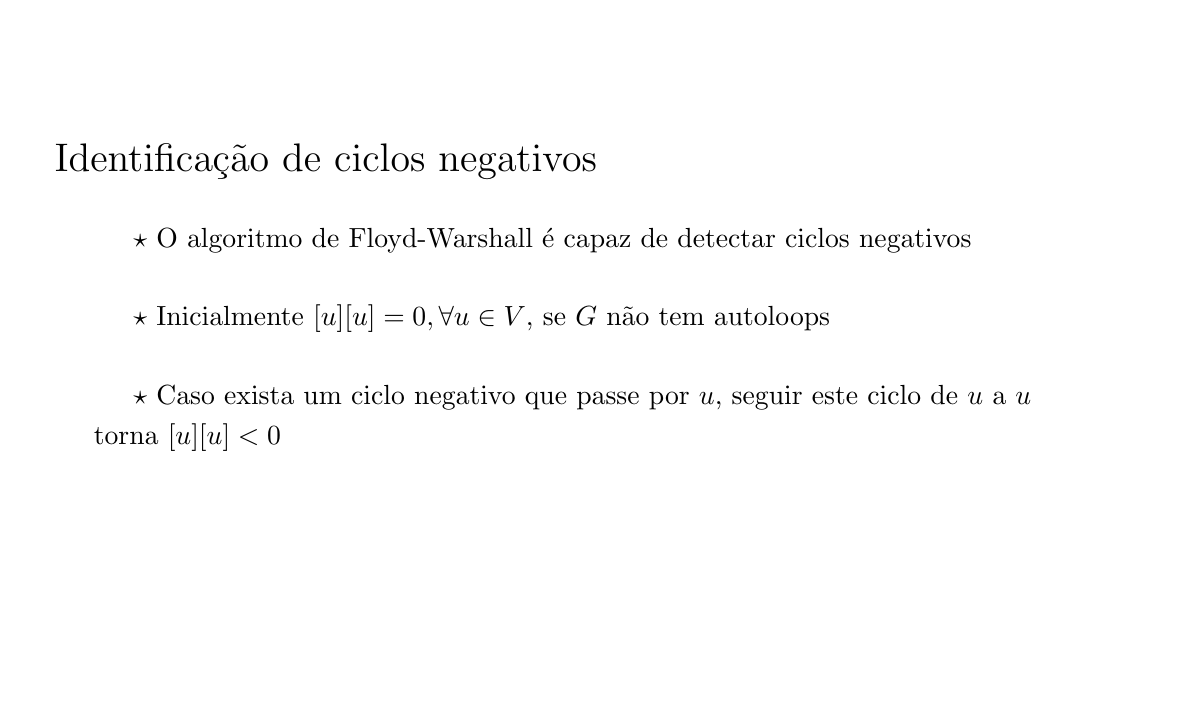
\begin{tikzpicture}
\node[draw,opacity=0] at (0, 0) {x};
\node[draw,opacity=0] at (14, 8) {x};

	\node[anchor=west] (title) at (0.0, 6.5) { \Large \bbbold{Identificação de ciclos negativos} };


	\node[anchor=west] (line1) at (1.0, 5.5) { $\star$ \bbtext{O algoritmo de Floyd-Warshall é capaz de detectar ciclos negativos} };


	\node[anchor=west] (line2) at (1.0, 4.5) { $\star$ \bbtext{Inicialmente $\dist[u][u] = 0, \forall u\in V$, se $G$ não tem \bbenglish{autoloops}} };



	\node[anchor=west] (line3) at (1.0, 3.5) { $\star$ \bbtext{Caso exista um ciclo negativo que passe por $u$, seguir este ciclo de $u$ a $u$} };

	\node[anchor=west] (line3a) at (0.5, 3.0) { \bbtext{torna $\dist[u][u] < 0$} };

\end{tikzpicture}
\end{frame}
\begin{frame}[plain,t]
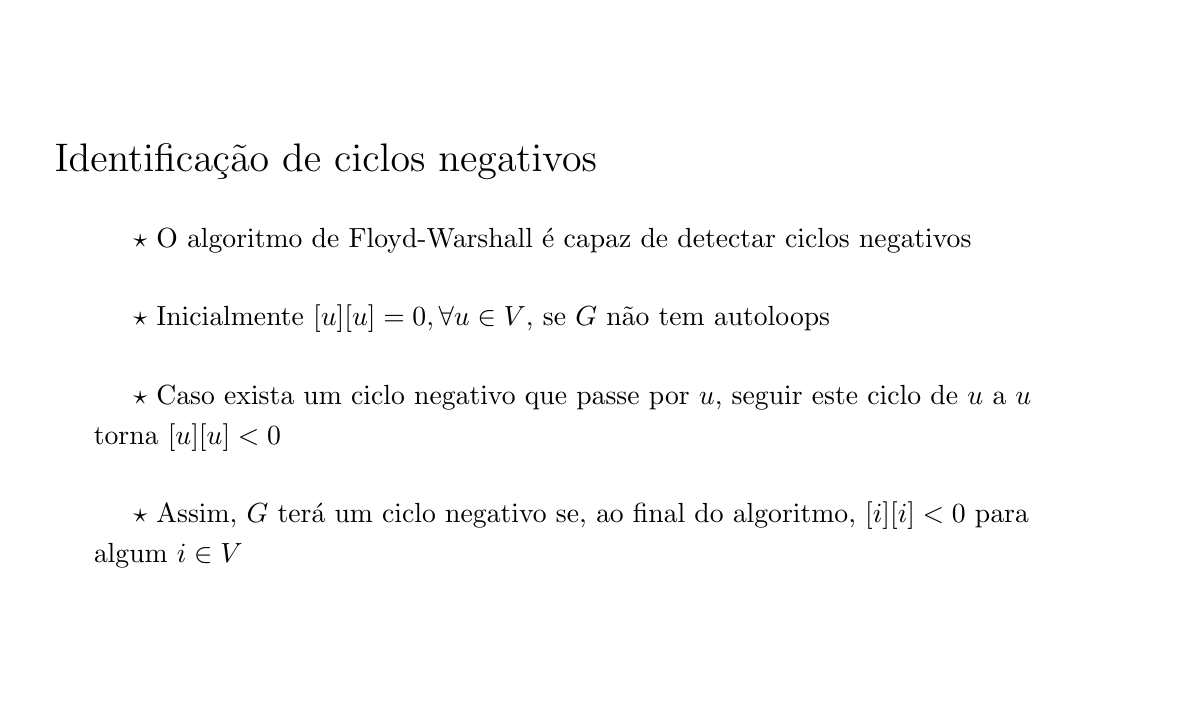
\begin{tikzpicture}
\node[draw,opacity=0] at (0, 0) {x};
\node[draw,opacity=0] at (14, 8) {x};

	\node[anchor=west] (title) at (0.0, 6.5) { \Large \bbbold{Identificação de ciclos negativos} };


	\node[anchor=west] (line1) at (1.0, 5.5) { $\star$ \bbtext{O algoritmo de Floyd-Warshall é capaz de detectar ciclos negativos} };


	\node[anchor=west] (line2) at (1.0, 4.5) { $\star$ \bbtext{Inicialmente $\dist[u][u] = 0, \forall u\in V$, se $G$ não tem \bbenglish{autoloops}} };



	\node[anchor=west] (line3) at (1.0, 3.5) { $\star$ \bbtext{Caso exista um ciclo negativo que passe por $u$, seguir este ciclo de $u$ a $u$} };

	\node[anchor=west] (line3a) at (0.5, 3.0) { \bbtext{torna $\dist[u][u] < 0$} };


	\node[anchor=west] (line4) at (1.0, 2.0) { $\star$ \bbtext{Assim, $G$ terá um ciclo negativo se, ao final do algoritmo, $\dist[i][i] < 0$ para} };

	\node[anchor=west] (line4a) at (0.5, 1.5) { \bbtext{algum $i\in V$} };

\end{tikzpicture}
\end{frame}
\begin{frame}[plain,t]

\inputsnippet{cpp}{11}{30}{codes/cycle.cpp}

\end{frame}
\begin{frame}[plain,t]
\begin{tikzpicture}
\node[draw,opacity=0] at (0, 0) {x};
\node[draw,opacity=0] at (14, 8) {x};

	\node[anchor=west] (title) at (0.0, 6.0) { \Large \bbbold{Problemas sugeridos} };

	\node[anchor=west] (a) at (1.0, 5.0) { $1.$ \bbtext{Codeforces Round \#179 (Div. 1) -- Problem B: Greg and Graph} };

	\node[anchor=west] (b) at (1.0, 4.0) { $2.$ \bbtext{LightOJ -- Travel Company} };

	\node[anchor=west] (c) at (1.0, 3.0) { $3.$ \bbtext{OJ 104 -- Arbitrage} };

	\node[anchor=west] (d) at (1.0, 2.0) { $4.$ \bbtext{OJ 10171 -- Meeting Prof. Miguel...} };

\end{tikzpicture}
\end{frame}
\begin{frame}[plain,t]

\begin{tikzpicture}
\node[draw,opacity=0] at (0, 0) {x};
\node[draw,opacity=0] at (14, 8) {x};

	\node[anchor=west] (title) at (0.0, 6.0) { \Large \bbbold{Referências} };

	\node[anchor=west] (a) at (1.0, 5.0) { $1.$ \bbtext{\bbbold{CP-Algorithms}. \bbenglish{Floyd-Warshall Algorithm}, acesso em 03/08/2021.} };

	\node[anchor=west] (b) at (1.0, 4.0) { $2.$ \bbbold{HALIM}, \bbtext{Felix}; \bbbold{HALIM}, \bbtext{Steve}. \bbenglish{Competitive Programming 3,} \bbtext{2010.} };

	\node[anchor=west] (c) at (1.0, 3.0) { $3.$ \bbbold{LAAKSONEN}, \bbtext{Antti}. \bbenglish{Competitive Programmer's Handbook,} \bbtext{2018.} };

	\node[anchor=west] (d) at (1.0, 2.0) { $4.$ \bbbold{SKIENA}, \bbtext{Steven}; \bbbold{REVILLA}, \bbtext{Miguel}. \bbenglish{Programming Challenges,} \bbtext{2003.} };

\end{tikzpicture}
\end{frame}
\end{document}
